\chaptertitle{Mesure de la topologie logique}
\label{chap:traceroute}
\introformatting

\lettrine{H}{istoriquement}, la topologie logique est celle qui a la première
fait l'objet de mesures massives. Les travaux de Faloutsos
\etal~\cite{FaloutsosFF99} et Pansiot \etal~\cite{280555} sur la topologie
logique ont initié toute une série d'opérations de mesure destinées à mesurer
cette topologie en utilisant des outils de diagnostic réseau. Le plus utilisé à
cet effet est sans aucun doute \traceroute. En principe, \traceroute permet
d'obtenir le chemin dans la topologie logique parcouru par un paquet envoyé
depuis la machine qui exécute \traceroute vers une cible donnée de la topologie
logique. L'utilisation massive de \traceroute a porté l'espoir d'établir des
cartes de la topologie logique en aggrégant des collectes de chemins. Mais de
nombreux travaux ont montré qu'en plus de problèmes techniques liés à l'outil
\traceroute~\cite{paristraceroute,pansiot2012,roughan201110}, la topologie
logique cartographiée est intrinsèquement
biaisée~\cite{LakhinaBCX03,AchlioptasCKM09,willinger,MDBP10,DallAstaABVV06,GuillaumeLM06,LatapyM08,roughan201110}.

Parce que la topologie logique et particulièrement l'utilisation de l'outil
\traceroute pour la mesurer sont au cœur de l'état de l'art, c'est sur cette
base que nous avons décidé de mener nos travaux préliminaires pour une première
mesure orientée propriété de la topologie d'Internet.

Notre première contribution a été d'analyser en détails le fonctionnement de
\traceroute et de mettre en évidence les confusions à l'origine d'erreurs
d'interprétation historiques de ses résultats (\refsec{traceroute-rigor}). En
surmontant ces confusions, nous avons mis au point une interprétation plus
restreinte de \traceroute, qui constitue notre primitive de mesure de bas niveau
(\refsec{traceroute-one-to-one}) qui permet d'obtenir une interface d'un voisin
d'une cible de la topologie \LLL.
Une utilisation distribuée de cette primitive de mesure de bas niveau nous a
permis de concevoir une primitive de mesure de haut niveau
(\refsec{traceroute-many-to-one}) qui permet d'obtenir, en principe, la liste
des interfaces extérieures de tous les voisins tournés vers le cœur d'un n\oe{}ud
quelconque d'Internet. Nous avons enfin conçu une procédure d'échantillonnage
(\refsec{traceroute-sampling}) et de correction d'erreurs
(\refsec{traceroute-filtering}) qui nous donne un premier moyen d'évaluer la
distribution de degré des routeurs du cœur dans la topologie logique à l'aide de
l'outil \traceroute. Le principe de cette méthode a été validé par des
simulations (\refsec{traceroute-simuls}). Enfin, pour attester de la faisabilité
pratique de notre méthode, nous l'avons expérimentée au cours d'une mesure
réelle depuis un ensemble de moniteurs du réseau Planetlab~\cite{planetlab}
(\refsec{traceroute-measurement}). Cette expérimentation nous a permis d'ajuster
la méthode à des contraintes expérimentales pour en déduire un protocole de
mesure (\refsec{traceroute-protocol}). Nous avons enfin pu positionner ces
travaux et leur contribution propre mais également déterminer leurs limites
(\refsec{traceroute-limits}).
Nous avons pu en tirer des conclusions importantes pour la suite de nos travaux
(\refsec{traceroute-conclusion}).

\section{Interprétation rigoureuse de \traceroute}
\label{sec:traceroute-rigor}

L'outil \traceroute est un utilitaire de diagnostic réseau utilisé
habituellement pour tenter d'identifier la liste des n\oe{}uds de la topologie
logique qui sont parcourus par les paquets \ip pour transiter d'un n\oe{}ud {\em
source} vers un n\oe{}ud {\em destination}. Il se base sur les RFC 1192\rfc{1122},
RFC 792\rfc{792}, et RFC 1812\rfc{1812}.

Les paquets \ip disposent d'un champ, {\em Time-to-Live} ou \ttl, qui indique
le nombre de {\em hops} autorisés qu'il reste au paquet. Ce compteur est
initialisé par l'expéditeur du paquet, normalement à des valeurs suffisamment élevée pour
atteindre sa destination dans des conditions régulières, par exemple 64 ou 128.
Chaque fois qu'un paquet traverse un n\oe{}ud, ce n\oe{}ud doit décrémenter la valeur
du \ttl de 1 avant de faire suivre le paquet. Si ce \ttl atteint 0, le n\oe{}ud
qu'il traverse doit supprimer le paquet, et renvoyer à l'expéditeur du paquet un
message \icmptimeout contenant un identifiant unique du paquet incriminé, pour
signaler un probable problème de routage. Ce mécanisme permet d'éviter que des
paquets piégés dans des boucles de routage n'emcombrent le réseau indéfiniment.

\traceroute exploite ce principe en forgeant des paquets avec des \ttl faibles
croissants, dans le but intentionnel de faire générer des messages \icmptimeout
à des routeurs à une {\em hop}-distance de leur point de départ donnée, en
chemin vers leur destination.

La \reffig{traceroute} illustre le fonctionnement de \traceroute. Supposons
qu'un moniteur ${\overline m} \in V_3$, (c'est à dire un hôte de la topologie
logique, \cf~\refdef{topologie-logique}) fabrique un paquet \ip d'identifiant
$p$ en indiquant dans l'en-tête sa propre adresse $m$ comme adresse
d'expédition, une adresse $t$ (pour {\em target}) d'une cible ${\overline t} \in
V_3$ comme adresse de destination, et une certaine valeur $n$ comme \ttl. Ce
paquet contient un message \icmp, \tcp ou \udp qui demande à la cible de
répondre qu'elle a bien réceptionné le paquet.

Le moniteur ${\overline m}$ envoie ce paquet $p$ d'identifiant $i$ et écoute
ensuite les paquets \icmptimeout et les messages de réponse de la cible. Si
${\overline m}$ reçoit un paquet de réponse, c'est que la cible a été atteinte
et le paquet a parcouru moins de $n$ {\em hops}. Si ${\overline m}$ ne reçoit
aucun paquet après un certain temps d'expiration ({\em timeout}), alors le
paquet d'origine est considéré comme perdu. Si ${\overline m}$ reçoit un paquet
\icmptimeout contenant l'identifiant $i$ d'origine, alors il lit l'adresse de
l'expéditeur de ce paquet \icmp, qui est celle d'une interface $r_n$ (adresse
\ip) d'un certain routeur $\overline{r_n} \in V_3$.
On peut alors supposer que le paquet $p$ a effectué $n$ {\em hops} en chemin
vers $t$ et a expiré en traversant $\overline{r_n}$. Dans la topologie logique,
cela signifie que le routeur $\overline{r_n}$ se trouve à une distance $n$ sur
un chemin entre ${\overline m}$ et ${\overline t}$.

\traceroute (\refalg{traceroute}) répète cette opération en partant
de $n = 1$ jusqu'à ce que la cible soit atteinte, c'est à dire si pour
un $n$ donné, il obtient une réponse appropriée de la part de la cible.
\traceroute affiche la liste de tous les n\oe{}uds ayant renvoyés des paquets
\icmptimeout, dans l'ordre des \ttl $n$ croissants.

\realfig{traceroute.png}{Fonctionnement de \traceroute} {Un moniteur ${\overline
m}$ possédant une interface $m$ envoie des paquets \ip avec des \ttl croissants
depuis 1 vers une cible ${\overline t}$ désignée par une interface $t$. Les
n\oe{}uds qui sont traversés pour atteindre $t$ génèrent des paquets \icmptimeout
qui permettent de les identifier.}{traceroute}

La nature exacte du paquet d'origine $p$ dépend du protocole de transport
(\LLLL) utilisé. S'il s'agit du protocole \icmp, alors le paquet contient un
message \icmp~{\sc Echo Request}. Si la cible répond à ce type de messages, ce
qui demande une configuration explicite et spécifique, alors elle répond avec un
paquet \icmp~{\sc Echo Reply}. Comme beaucoup de routeurs et d'hôtes sont
configurés pour {\em ne pas} répondre aux paquets \icmp~{\sc Echo Request}, on
peut alternativement utiliser des sondes \tcp ou \udp. Les sondes \tcp utilisent
des paquets \tcp~{\sc SYN} qui réclament l'ouverture d'une connexion \tcp, à
laquelle la cible répond avec un paquet \tcp~{\sc ACK}. Les sondes \udp sont
adressées à un port aléatoire \apriori inutilisé, pour que la cible réponde avec
un paquet \icmp~{\sc Destination Unreachable} indiquant que ce port ne peut être
atteint.

\begin{algorithm}
\caption{\traceroute}
\label{alg:traceroute}
\begin{algorithmic}
\Function{GénérerDemandeRéponse}{transport, port = {\sc null}}
\If{transport $==$ {\sc ICMP}}
	\State {\sc renvoyer} \icmp({\sc Echo Request})
\ElsIf{transport $==$ {\sc UDP}}
	\State {\sc renvoyer} \udp({\bf port} = port, {\bf corps} = {\sc RandomBytes}())
\ElsIf{transport $==$ {\sc TCP}}
	\State {\sc renvoyer} \tcp({\bf port} = port, {\bf corps} = {\sc SYN})
\EndIf
\EndFunction
\Procedure{EnvoyerSonde}{transport, port = {\sc null}, identifiant,
destinataire, TTL} \State e $\gets$ \textsc{EntêteIP}(\textbf{expediteur} =
\textsc{HostAddress}, \textbf{destinataire} = destinataire,
\textbf{identifiant} = identifiant, \textbf{TTL} = TTL)
\State c $\gets$ \Call{GénérerDemandeRéponse}{transport, port}
\State {\em
paquet} $\gets$ \Call{PaquetIP}{\textbf{EnTête} = e,
\textbf{Corps} = c}
\State \Call{EmettrePaquetIP}{{\em paquet}}
\EndProcedure
\Procedure{traceroute}{destinataire, transport, port = {\sc null}, timeout}
\State $n \gets 1$
\State \Call{Print}{``\traceroute depuis `` {\sc HostAddress} `` vers ``
destinataire ``:``}
\Loop
	\State identifiant $\gets$ {\sc RandomBytes()}
	\State \Call{envoyer-sonde}{transport, identifiant, destinataire, $n$}
	\State réponse $\gets$ \Call{AttendreRéponse}{{\bf type} = {\sc
	TimeExceeded}, {\bf identifiant} = identifiant, {\bf timeout} = timeout}
	\If{{\sc Type}(réponse) $==$ {\sc CibleAtteinte}(transport)}
		\State \Call{Print}{``Cible `` destinataire `` atteinte après `` n `` hops''}
		\State {\sc Exit()}	
	\ElsIf{{\sc Type}(réponse) $==$ {\sc Timeout}}
		\State \Call{Print}{``\hop `` n `` $\rightleftarrows$ '' {\sc
		Expéditeur}(réponse)}
	\Else
		\State \Call{Print}{``\hop `` n `` $\rightleftarrows$ *}
	\EndIf
	\State $n \gets n + 1$
\EndLoop
\EndProcedure
\end{algorithmic}
\end{algorithm}

Le bon fonctionnement de \traceroute suppose que les sondes peuvent à la fois
parvenir à la cible et aux n\oe{}uds intermédiaires, et que les paquets
\icmptimeout et les paquets de réponse en provenance de la cible (dépendant du
type de transport choisi) soient correctement générés et soient capables de
parvenir au moniteur à leur tour. Les messages \icmp~{\sc Echo Request} sont
très souvent ignorés, puisqu'ils n'ont pas d'autre utilité propre que le
diagnostic et sont parfois considérés comme des atteintes à la sécurité. En
revanche, les sondes \tcp et \udp sont indiscernables de paquets correspondant à
un fonctionnement ``normal'' (à l'exception de leur \ttl très faible). Certains
{\em firewalls}, cependant, considèrent qu'un paquet avec un \ttl trop faible
(inférieur à 10, par exemple) est suspect et le rejettent. Enfin, certains
routeurs et {\em firewalls} bloquent complètement le traffic \icmp, ce qui
empêche les réponses \icmptimeout de parvenir au moniteur.
Pour des raisons de sécurité analogue, certaines cibles ne répondent pas de
paquets \icmp~{\sc Destination Unreachable} aux sondes \udp, ou refusent
d'accepter des connexions \tcp (donc de répondre aux sondes \tcp) qu'elles
n'ont pas au préalable autorisées.

Lorsque \traceroute fonctionne correctement, c'est à dire que le traffic n'est
pas bloqué, il fournit donc une liste $(r_1, \ldots, r_n, t)$ d'adresses \ip où
$r_k$ correspond à la réponse pour le $k$-ième {\em hop}.

L'{\em interprétation classique de \traceroute}, à la base de la plupart des
travaux de cartographie au niveau \ip, est souvent équivalente, de manière
implicite, à la formulation suivante:

\begin{hypothese}[Interprétation classique de \traceroute] La liste $(r_1,
\ldots, r_n, t)$ produite par \traceroute depuis $m$ vers $t$ correspond à la
{\em trace} d'une certaine {\em route} parcourue par les sondes
(\cf~\refdef{route}), donc par les paquets \ip, pour atteindre $t$ depuis $m$
(d'où le nom de l'utilitaire, \traceroute), et chaque paire $\{r_k, r_{k+1}\}$
est donc un lien entre deux interfaces au niveau \LLL.
\label{hyp:traceroute-classique}
\end{hypothese}

À la lumière du formalisme que nous avons introduit, cette interprétation
apparaît très inexacte, sans même parler des effets liés à la dynamique. 

Elle repose notamment sur une confusion entre les {\em n\oe{}uds} \LLL traversés
par les paquets (chaque $\overline{r_k}$), et les {\em interfaces} utilisées par
ces n\oe{}uds pour répondre (chaque $r_k$).
Cette confusion pourrait être légitime dans deux cas: (1) dans le cas où chaque
$\overline{r_k}$ ne dispose que d'une seule interface connectée à Internet,
ou (2) dans le cas où chaque $\overline{r_k}$ utilise toujours la même
interface ($\overline{r_k}$) pour répondre à \traceroute, {\em dans tous les cas}.

Le cas (1) est au mieux très rare. Supposons qu'un routeur $\overline{r_k}$
dispose d'une unique adresse \ip $r_k$. Alors soit $\overline{r_k}$ est de degré
1 dans la topologie \LLL, soit toutes ses connexions au niveau \LLL se font par
l'intermédiaire d'une entité de niveau \LL qui n'est pas une entité de niveau
\LLL. Si $\overline{r_k}$ n'est pas de degré 1, alors l'entité de niveau \LL
intermédiaire qui n'est pas de niveau \LLL est assimilable topologiquement à un
\switch. Or, de très nombreux routeurs ne sont ni de degré 1 au niveau logique,
ni connectés exclusivement à travers l'intermédiaire d'un \switch.
L'approximation résultant de (1) est donc fausse dans tous ces cas là.

Examinons à présent le cas (2). Une adresse $r_k$ apparaît dans le résultat de
\traceroute depuis $m$ vers $t$ si un certain routeur $\overline{r_k}$ a envoyé
un message \icmptimeout en direction de $m$ en utilisant pour cela l'interface
$r_k$. $r_k$ est donc l'interface {\em choisie par $\overline{r_k}$} pour router
un message \icmp à destination de $m$. Il y a ici également deux sous-cas
possibles: soit $\overline{r_k}$ est configuré pour utiliser {\em toujours} sa
même interface $r_k$ pour générer des messages \icmptimeout, soit l'interface
$r_k$ choisie dépend d'une manière ou d'une autre de $m$ et éventuellement
d'autres paramètres.
Certains routeurs sont en effet configurés pour adopter le premier comportement. Mais cela ne peut être
le cas général, et la rareté de cette configuration a été démontrée
expérimentalement dans plusieurs travaux liés à l'{\em
anti-aliasing}~\cite{keys2010internet, alias-bias}. Le seul cas possible restant
dans le cas général est donc le suivant: l'interface choisie par
$\overline{r_k}$ pour envoyer le paquet \icmptimeout à $m$ dépend de $m$, et
éventuellement d'autres paramètres.
Informellement, cela signifie que pour répondre à une sonde \traceroute,
$\overline{r_k}$ utilise une interface ``tournée vers $m$'', ou du moins une
interface spécifiquement choisie pour envoyer un message vers $m$.

Les conséquences de cette interprétation abusive vont bien au delà d'une simple
considération formelle: elles conduisent à supposer l'existence de liens en
réalité inexistants, même dans des cas très simples. Supposons (comme illustré
en \reffig{traceroute-classique}) que deux hôtes terminaux ({\em end hosts}) $m$
et $t$ soient connectés à travers un routeur $\overline{r}$ possédant deux
interfaces $\overline{r_m}$ et $\overline{r_t}$, la première connectée à
$\overline{m}$ et l'autre à $\overline{t}$.
La seule route depuis $\overline{r}$ vers $m$ passe donc par l'interface $r_m$.
En exécutant \traceroute depuis $m$ vers $t$, on obtient en principe la sortie
suivante :

\begin{center}
\begin{tabularx}{0.8\textwidth}{|X|}
\hline
\vspace{0 mm} \hspace{5 mm} \texttt{\traceroute depuis \(m\) vers \(t\):} \\
\hspace{5 mm} \texttt{\hop 1 \(\rightleftarrows r_m\)} \\
\hspace{5 mm} \texttt{Cible \(t\) atteinte après 2 hops.}
\vspace{3 mm}  \\
\hline
\end{tabularx}
\end{center}

Alors d'après~\refhyp{traceroute-classique}, il doit exister un lien $(r_m, t)$,
ce qui n'est pas vrai.

\realfig{traceroute-classique.png}{Erreurs dans l'interprétation de
\traceroute}{$m$ envoie un \traceroute vers $t$. La première sonde est
réceptionnée par $\overline{r}$ qui répond avec son interface $r_m$.
L'interprétation classique suppose l'existence d'un lien inexistant entre $r_m$
et $t$.}{traceroute-classique}

Ce premier défaut dans l'interprétation classique de \traceroute peut toutefois
être corrigé, si on l'exprime correctement en termes de n\oe{}uds \LLL plutôt qu'en
termes d'interfaces. Cette hypothèse corrigée est la suivante:

\begin{hypothese}[Interprétation classique de \traceroute (corrigée)] Soit la
liste $(r_1, \ldots, r_n, t)$ produite par \traceroute depuis $m$ vers $t$.
Alors pour chaque $k$, $\{\overline{r_k},\overline{r_{k+1}}\} \in E_3$, c'est à
dire que $\overline{r_k}$ et $\overline{r_{k+1}}$ sont voisins au niveau logique
puisqu'une sonde passe de $\overline{r_k}$ à $\overline{r_{k+1}}$ en un {\em
hop}.
\label{hyp:traceroute-classique-corr}
\end{hypothese}

Mais plusieurs travaux
antérieurs~\cite{paristraceroute,willinger,SherwoodBS08,SpringMWA04,VigerACMLFT08,AugustinCOVFLMT06}
ont montré que même cette interprétation est fausse dans de nombreux cas, à
cause de la dynamique des routes et notamment celle induite par l'équilibrage de
charge.
Supposons (comme illustré en \reffig{traceroute-loadbalancing}) par exemple que
${\overline m}$ soit connecté à un routeur ${\overline r_1}$, lui-même connecté
à deux routeurs ${\overline r_2}$ et ${\overline r_3}$.
${\overline r_2}$ est connecté à un routeur ${\overline r_4}$ connecté à
$\overline{t}$ mais pas à ${\overline r_3}$, et ${\overline r_3}$ est connecté à
un routeur ${\overline r_5}$ connecté à ${\overline t}$ mais pas à ${\overline r_4}$. Si
${\overline r_2}$ pratique l'équilibrage de charge ({\em load-balancing}), par
exemple en envoyant un paquet sur deux à destination de $t$ vers $r_2$ et $r_3$
alternativement, alors \traceroute peut fournir la sortie suivante:

\begin{center}
\begin{tabularx}{0.8\textwidth}{|X|}
\hline
\vspace{0 mm} \hspace{5 mm} \texttt{\traceroute depuis \(m\) vers \(t\):} \\
\hspace{5 mm} \texttt{\hop 1 \(\rightleftarrows r_1\)} \\
\hspace{5 mm} \texttt{\hop 2 \(\rightleftarrows r_2\)} \\
\hspace{5 mm} \texttt{\hop 1 \(\rightleftarrows r_5\)} \\
\hspace{5 mm} \texttt{Cible \(t\) atteinte après 4 hops.}
\vspace{3 mm}  \\
\hline
\end{tabularx}
\end{center}

Alors d'après~\refhyp{traceroute-classique-corr}, ${\overline r_2}$ est un
voisin de ${\overline r_5}$ au niveau logique, ce qui n'est pas vrai.
(\reffig{traceroute-loadbalancing})

\realfig{traceroute-loadbalancing.png}{Erreurs dans l'interprétation de
\traceroute, même corrigée} {$\overline{m}$ envoie un \traceroute vers $t$ en
utilisant son interface $m$, en passant par ${\overline r_1}$ qui effectue de
l'équilibrage de charge.
\traceroute indique successivement $r_2$ et $r_5$ dans sa sortie, pourtant
${\overline r_2}$ et ${\overline r_5}$ ne sont pas voisins.
Les liens réels sont indiqués en traits pleins, le lien inexistant suggéré par
\traceroute est en pointillés.} {traceroute-loadbalancing}

Si pour ces raisons il semble peu vraissemblable de valider une hypothèse de
haut niveau sur les résultats de \traceroute, on peut toutefois se référer à la
description rigoureuse que nous avons donné de son fonctionnement pour formuler
une hypothèse à un plus bas niveau qui découle directement de cette description:

\begin{hypothese}[Interprétation bas niveau de \traceroute] Soit $(r_1, \ldots,
r_n, t)$ le résultat de \traceroute depuis $m$ vers $t$.
Alors pour chaque $k$, $r_k$ est une interface d'un certain n\oe{}ud
$\overline{r_k}$ de \LLL, qui se trouve sur {\em une} route depuis $m$ vers $t$
à une {\em hop}-distance $k$ de $m$. Chaque $r_k$ dépend de $m$ et éventuellement
d'autres paramètres.
\label{hyp:traceroute-realiste}
\end{hypothese}

Nous allons maintenant voir comment exploiter cette hypothèse pour mesurer une
information fiable et pertinente sur une cible $t$ à partir d'un moniteur $m$.

\section{Primitive de mesure de bas niveau basée sur \traceroute}
\label{sec:traceroute-one-to-one}

Nous avons exposé (\refsec{traceroute-rigor}) une interprétation réaliste
(\refhyp{traceroute-realiste}) du résultat de \traceroute depuis un moniteur
$\overline{m}$ à travers une interface $m$ vers une cible $\overline{t}$
désignée par une adresse $t$. Nous avons en outre montré qu'il était difficile
d'exploiter ce résultat pour opérer des déductions sur d'éventuels liens {\em
entre les n\oe{}uds intermédiaires} donnés par \traceroute, en particulier car les
sondes successives peuvent emprunter des routes différentes. Pour cette raison,
nous avons décidé de nous intéresser uniquement aux informations données par le
{\em dernier résultat donné par \traceroute avant d'atteindre la cible}. Dans ce
chapitre, nous utiliserons ainsi la notation suivante:

\begin{definition}[Observation d'une cible depuis un moniteur] Soit $(r_1,
\ldots, r_n, t)$ le résultat de \traceroute depuis $m$ vers $t$. On note $m(t) =
r_n \in \IPSet$\footnote{Par conséquent, $\overline{m(t)} = \overline{r_n} \in
V_3$} et on l'appelle {\em observation de $t$ depuis $m$}.
\label{def:traceroute-one-to-one}
\end{definition}

Alors d'après \refhyp{traceroute-realiste}, $m(t)$ est une interface d'un
certain routeur $\overline{m(t)}$ qui se trouve à une {\em hop}-distance $n$ de
$m$ en chemin vers $t$, tandis que $t$ se trouve à une {\em hop}-distance $n+1$
de $m$. Plus précisément, il s'agit de l'interface choisie par $\overline{m(t)}$
pour envoyer un paquet \icmptimeout vers $m$.

Supposons temporairement que {\em toutes les sondes envoyées par \traceroute
depuis $m$ vers $t$} empruntent la même route. Alors $\overline{m(t)}$ est
nécessairement un voisin de $\overline{t}$ dans la topologie logique, et plus
précisément la dernière sonde \traceroute (celle qui atteint $t$) passe en un
{\em hop} de $\overline{m(t)}$ à $\overline{t}$
(\reffig{traceroute-one-to-one-simple}). Ce cas simple suggère la manière
dont nous allons tenter d'interpréter $\overline{m(t)}$ comme un voisin au niveau
logique de $\overline{t}$.

\realfig{traceroute-one-to-one-simple.png}{Observation d'une cible depuis un
moniteur} {$\overline{m}$ lance un \traceroute vers $t$ en utilisant son
interface $m$, et toutes les sondes empruntent la même route. Alors
$\overline{r_n} = \overline{m(t)}$ est nécessairement un voisin de
$\overline{t}$.} {traceroute-one-to-one-simple}

Mais comme nous l'avons déjà évoqué (\refsec{traceroute-rigor}),
toutes les sondes de \traceroute n'empruntent pas nécessairement la même route.
En revanche, il suffit que les deux dernières sondes de \traceroute empruntent
des routes {\em de même longueur}: même dans le cas d'un changement de route
entre ces deux sondes, l'information de la longueur totale de la route empruntée
suffit à conclure que $\overline{m(t)}$ est un voisin au niveau logique de
$\overline{t}$ (\reffig{traceroute-one-to-one-favorable}). En particulier:

\begin{proposition}[Interprétation de l'observation d'un moniteur vers une
cible] Si toutes les routes depuis $m$ vers $t$ ont la même longueur, alors
$\overline{m(t)}$ est un voisin au niveau logique de $\overline{t}$.
\label{prop:traceroute-one-to-one}
\end{proposition}

\realfig{traceroute-one-to-one-favorable.png}{Observation d'une cible depuis un
moniteur, cas favorable} {$\overline{m}$ lance un \traceroute vers $t$ en
utilisant son interface $m$. Deux routes différentes sont parcourues
alternativement par les sondes, mais ces deux routes font la même longueur. On
peut conclure que $\overline{m(t)} = \overline{r_5}$ est bien un voisin de
$\overline{t}$.} {traceroute-one-to-one-favorable}

Inversement, en revanche, si les deux dernières sondes de \traceroute (celle qui
provoque l'observation de $m(t)$, et celle qui atteint $\overline{t}$)
empruntent des routes de longueur différentes, $\overline{m(t)}$ peut très bien
ne {\em pas} être voisin de $\overline{t}$. Le cas le plus simple est celui de
l'équilibrage de charge entre deux sous-routes de longueur distincte. Soit par
exemple (comme illustré en \reffig{traceroute-one-to-one-defavorable}) un
moniteur $\overline{m}$ connecté à un certain routeur $\overline{r_1}$. Ce
routeur est connecté à deux autres routeurs $\overline{r_2}$ et
$\overline{r_3}$. $\overline{r_3}$ est connecté directement à $\overline{t}$,
tandis que $\overline{r_2}$ est connecté à un autre routeur $\overline{r_4}$,
qui lui est connecté à $\overline{t}$. Appelons $\overline{R}$ la route qui
relie $\overline{m}$ à $\overline{t}$ en empruntant $(\overline{r_1},
\overline{r_3}, \overline{t})$. Appelons $\overline{R'}$ la route empruntant
$(\overline{r_1}, \overline{r_2}, \overline{r_4}, \overline{t})$. $\overline{R}$
est de longueur 3, et $\overline{R'}$ est de longueur 4. Si $\overline{r_1}$
pratique un équilibrage de charge uniforme entre $\overline{r_2}$ et
$\overline{r_3}$, alors \traceroute peut renvoyer la liste $(\overline{r_1},
\overline{r_2}, \overline{t})$. Dans ce cas, $\overline{m(t)} = \overline{r_2}$,
alors que $\overline{r_2}$ n'est {\em pas} un voisin de $\overline{t}$.

\realfig{traceroute-one-to-one-defavorable.png}{Observation d'une cible depuis
un moniteur, cas défavorable} {$\overline{m}$ lance un \traceroute vers $t$ en
utilisant son interface $m$.
Deux routes différentes sont parcourues alternativement par les sondes, mais ces deux routes
n'ont pas la même longueur. Dans ce cas, $\overline{m(t)} = \overline{r_2}$
n'est {\em pas} un voisin de $\overline{t}$. En pointillés, le lien inexistant
entre $\overline{r_2}$ et $\overline{t}$.}{traceroute-one-to-one-defavorable}

Nous adresserons la problématique de détecter le cas défavorable où les routes
entre un moniteur et une cible sont de longueur variable ultérieurement
(\refsec{traceroute-filtering}). Pour l'instant, nous noterons:

\begin{definition}[Ensemble des moniteurs observant correctement une cible] On
appelle {\em ensemble des moniteurs observant correctemment une cible $t$}
l'ensemble $\mathbb{M}(t)$ des moniteurs depuis lesquels toutes les routes vers
$t$ sont de même longueur; en particulier tels que $\overline{m(t)}$ est un
voisin de $\overline{t}$.
\end{definition} 

Pour une certaine cible $t \in \IPSet$, nous considérons alors que $m \in
{\mathbb{M}(t)} \mapsto m(t) \in \IPSet$ est notre {\em primitive de bas niveau
basée sur \traceroute}.

\section{Primitive de mesure de haut niveau basée sur \traceroute}
\label{sec:traceroute-many-to-one}

Nous avons vu (\refsec{traceroute-one-to-one}) que nous pouvons utiliser une
interprétation très prudente de \traceroute pour mesurer, à l'aide d'un moniteur
$m \in \mathbb{M}(t)$, une interface $m(t)$ d'un voisin au niveau logique d'une
certaine cible $t$. Nous avons également noté que sauf dans le cas d'une
configuration explicite imposant à un routeur d'utiliser toujours la même
interface pour envoyer des paquets \icmptimeout, le choix de l'interface $m(t)$
par $\overline{m(t)}$ dépend de $m$ (donc de $\overline{m}$) et éventuellement
d'autres paramètres (tels qu'un équilibrage stochastique).
Enfin, évidemment, $\overline{m(t)}$ dépend de $m$ (donc de $\overline{m}$)
puisqu'il dépend des routes empruntées par les sondes \traceroute depuis $m$
vers $t$.

Soient alors $\overline{m} \in \mathbb{M}(t), \overline{m'} \in \mathbb{M}(t)$
deux moniteurs {\bf distincts}. Il est possible que $m(t) \neq m'(t)$.
Deux cas sont possibles: (1) $\overline{m(t)} = \overline{m'(t)}$ ou (2)
$\overline{m(t)} \neq \overline{m'(t)}$. Le cas (1) se présente lorsque $m$ et
$m'$ observent deux interfaces distinctes d'un même routeur. Le cas (2) se
présente lorsque les routes empruntées par les sondes \traceroute depuis $m$ et
$m'$ atteignent $\overline{t}$ par des voisins différents
(\reffig{traceroute-two-to-one}).

\realfig{traceroute-two-to-one.png}{Observation d'une cible depuis deux
moniteurs} {En haut, (1):
les sondes \traceroute atteignent $\overline{t}$ par le même voisin
$\overline{r} = \overline{m(t)} = \overline{m'(t)}$ mais $\overline{r}$ utilise
deux interfaces différentes $m(t)$ et $m'(t)$ pour y répondre. En bas, (2): les
sondes \traceroute atteignent $\overline{t}$ par des voisins distincts de
$\overline{t}$ et donc $\overline{m(t)} \neq \overline{m'(t)}$.}
{traceroute-two-to-one}

En utilisant \traceroute vers une même cible $\overline{t}$ désignée par l'une
de ses adresses $t$ depuis deux moniteurs, on peut donc collecter davantage
d'information sur les voisins logiques de $\overline{t}$. Nous généralisons ce
principe avec un ensemble arbitraire de moniteurs:

\begin{definition}[Observation d'une cible depuis un ensemble de moniteurs] Soit
$M = \{m_1, \ldots m_n\}$ un ensemble d'interfaces appartenant chacune à des
moniteurs $\overline{M} = \{\overline{m_1}, \ldots, \overline{m_n}\} \subset
\mathbb{M}(t)$.
On note $M(t) = \{m_1(t), \ldots, m_n(t)\}$ et $\overline{M(t)} =
\{\overline{m_1(t)}, \ldots, \overline{m_n(t)}\}$. On appelle $M(t)$ {\em
observation de $t$ depuis $M$}.
\label{def:traceroute-many-to-one}
\end{definition}

Par construction, puisque $M \subset \mathbb{M}(t)$, alors $\overline{M(t)}$ est
un ensemble de voisins au niveau logique de $\overline{t}$ et en particulier,
$|\overline{M(t)}| \leq d_3(\overline{t})$.
Nous allons examiner les conditions sur $m$ et $t$ pour que $\overline{M(t)}$
soit le plus grand possible. Plus précisément, nous allons tenter de déterminer
sous quelles conditions sur $M$ et $t$ on peut observer {\em tous} les voisins
de $\overline{t}$, c'est à dire que $|\overline{M(t)}| = d_3(\overline{t})$.

Remarquons d'abord que cette condition dépend à la fois de $M$ et de $t$.
Puisque chaque moniteur $m$ observe au plus {\em une seule} interface d'{\em un
seul} voisin de $\overline{t}$, alors $|\overline{M(t)}| \leq |M|$ (le cas
d'égalité survient lorsque chaque moniteur observe une interface d'un voisin
différent). En particulier, si $|M| < d_3(\overline{t})$, la condition n'est pas
réalisable. On doit donc {\em au minimum} disposer de davantage de moniteurs que
le degré de la cible.

Mais il ne suffit pas d'avoir un grand nombre de moniteurs: il faut également
qu'ils soient positionnés correctement par rapport à la cible, et à ses voisins,
pour qu'on puisse tous les observer à l'aide des sondes \traceroute. Supposons
(comme illustré en \reffig{traceroute-impossible}) par exemple qu'un certain
voisin de $\overline{t}$ soit un n\oe{}ud de degré 1, c'est à dire que son seul
voisin est $\overline{t}$. Alors quel que soit l'ensemble des moniteurs $M$, il
est impossible d'observer ce voisin à l'aide de sondes \traceroute.

\realfig{traceroute-impossible.png}{Voisin impossible à observer avec
\traceroute} {La cible $\overline{t}$ est voisine d'un n\oe{}ud $\overline{r}$ de
degré 1. Même si tous les autres n\oe{}uds du graphe sont des moniteurs, alors il
est impossible d'observer $\overline{r}$ avec \traceroute.}
{traceroute-impossible}

Nous allons généraliser ce principe en définissant, pour une cible $t \in
\overline{t}$ donnée et l'un de ses voisins $\overline{v}$, l'ensemble des
n\oe{}uds qui sont capables d'observer $\overline{v}$ en ciblant $t$.

\begin{definition}[N\oe{}uds capables d'observer un voisin donné d'une cible] Soit
$t \in \overline{t}$ une cible et $\overline{v} \in V(\overline{t})$. On note
$\mathbb{M}(\overline{t}, \overline{v})$ l'ensemble des n\oe{}uds $\overline{u}$
tels qu'il existe un chemin de $\overline{u}$ vers $\overline{t}$ qui passe par
$\overline{v}$. On appelle cet ensemble l'{\em
ensemble des n\oe{}uds capables d'observer $\overline{v}$}.
\end{definition}

En particulier, puisque $\overline{u(t)}$ se trouve sur un chemin de
$\overline{u}$ à $\overline{t}$ ne passant pas par $\overline{t}$, alors
$\overline{u(t)} = \overline{v} \Rightarrow \overline{u} \in
\mathbb{M}(\overline{t}, \overline{v})$. Nous allons tenter de caractériser cet
ensemble plus en détails.

On partitionne les topologies d'Internet en deux sous-ensemble de n\oe{}uds
complémentaires, le {\em cœur} et le {\em bord} d'Internet (illustré en
\reffig{traceroute-core-border}), ainsi définis :

\begin{definition}[Cœur et bord d'Internet] Soit $(U_n)$ la suite telle que
$U_0 = V_3$ et $U_{n+1}$ est l'ensemble des n\oe{}uds de degré $> 1$ dans $U_n$
(c'est à dire dans le sous-graphe de $G_3$ dont les liens ont leurs deux
extrémités dans $U_n$).
On note $C_3$ et on appelle le {\em cœur de la topologie logique} la limite
(finie) de $(U_n)$. On note $B_3$ et on appelle le {\em bord de la topologie
logique} l'ensemble $V_3 \setminus C_3$.
\end{definition}

Moins formellement, le cœur de la topologie logique d'Internet $C_3$ correspond
à l'ensemble des n\oe{}uds d'Internet dont on a retiré récursivement les n\oe{}uds de
degré 1, ou de manière équivalente dont on a retiré récursivement les arbres. Le
bord correspond aux n\oe{}uds ainsi retirés.

\realfig{traceroute-core-border.png}{Cœur et bord d'Internet} {On retire
récursivement les n\oe{}uds de degré 1 d'un graphe. Chaque n\oe{}ud du {\em
bord} est marqué par un nombre $k$, qui correspond à l'itération à laquelle il
est supprimé. Les n\oe{}uds restants (en noir) sont les n\oe{}uds du {\em
cœur}.} {traceroute-core-border}

Nous pouvons ainsi définir deux notions très importantes pour caractériser les
voisins d'une certaine cible $t \in \overline{t}$ par rapport à la mesure:

\begin{definition}[Arbre enraciné, fils et parent dans un arbre enraciné]
Soit $A$ un arbre et $u$ un n\oe{}ud de $A$. On appelle {\em arbre enraciné} de
racine $u$ le couple $(A, u)$ qu'on note $A(u)$, et on dit alors que $u$ est la
racine de cet arbre. Soit $v$ un n\oe{}ud de $A(u)$, et $w$ un voisin de $u$. Il
y a alors deux possibilités qui s'excluent mutellement : soit (1) $v$ est sur
l'unique chemin de $u$ vers $w$, soit (2) $w$ est sur l'unique chemin de $u$
vers $v$. Dans le premier cas, on dit que $v$ est le {\em parent} de $w$. Dans
le deuxième cas, on dit que $v$ est un {\em fils} de $w$.
\end{definition}

\begin{definition}[Voisinage d'une cible tourné vers le bord, degré dans le
bord] Soit un n\oe{}ud $\overline{t} \in V_3$. Notons $C_3(\overline{t}) =
V(\overline{t}) \cap C_3$ et $B_3(\overline{t}) = V(\overline{t}) \cap B_3$.
Soit $A(\overline{t})$ l'arbre enraciné de racine $\overline{t}$. On appelle
{\em voisinage de $\overline{v}$ tourné vers le bord} les n\oe{}uds de
$B_3(\overline{t})$ qui sont également des fils de $\overline{t}$ dans
$A(\overline{t})$ et on note $B_3(V(\overline{t}))$ cet ensemble. On note
$d_{B_3}(\overline{t}) = |B_3(V(\overline{t}))|$ et on appelle cette valeur le
{\em degré dans le bord} de $\overline{t}$.
\end{definition}

\begin{definition}[Voisinage d'une cible tourné vers le cœur, degré dans le
cœur] Soit un n\oe{}ud $\overline{t} \in V_3$. On appelle {\em voisinage de
$\overline{t}$ tourné vers le cœur} l'ensemble
$C_3(V(\overline{t})) = V(\overline{t}) \setminus B_3(V(\overline{t}))$. Si
$\overline{t} \in C_3$, alors $C_3(V(\overline{t})) = C_3(\overline{t})$. On
note $d_{C_3}(\overline{t}) = |C_3(V(\overline{t}))|$ et on appelle cette valeur
le {\em degré dans le cœur} de $\overline{t}$.
\end{definition}

% Notons que ces deux notions n'ont d'intérêt que si au moins certains des voisins
% de $\overline{t}$ sont dans le bord. En effet, si tous les voisins de
% $\overline{t}$ sont dans le cœur, alors tous les voisins de $\overline{t}$ sont
% {\em tournés vers le cœur} (puisqu'alors $A(\overline{t})$ est réduit à sa
% racine $\overline{t}$).

Si un certain voisin $\overline{v} \in V(\overline{t})$ est dans le cœur, il ne
peut pas être un fils de $\overline{t}$ dans $A(\overline{t})$, sinon il serait
lui-même racine d'un sous-arbre de $A(\overline{t}))$ et il serait donc dans le
bord. Donc si $\overline{v}$ est dans le cœur, il appartient nécessairement au
voisinage tourné vers le cœur de $\overline{t}$. Soit alors un voisin
$\overline{v}$ de $\overline{t}$ dans le bord. Il y a deux cas possibles: soit
$\overline{t}$ est lui-même dans le bord (1), soit $\overline{t}$ est dans le
cœur (2).

Si $\overline{t}$ est dans le bord (1), alors soit $\overline{v} \in
C_3(V(\overline{t}))$ (1.a), soit $\overline{t} \in B_3(V(\overline{v}))$ (1.b).
On peut alors déduire $\mathbb{M}(t, \overline{v})$. Dans le cas (1.a), tous les
chemins depuis $\overline{v}$ vers le cœur passent par $\overline{t}$, donc
$\mathbb{M}(t, \overline{v})$ est exactement l'ensemble des n\oe{}uds qui sont
eux-mêmes des descendants de $\overline{v}$ dans l'arbre enraciné
$A(\overline{v})$. Dans le cas (1.b), c'est la situation inverse: tous les
chemins depuis $\overline{t}$ vers le cœur passent par $\overline{v}$, et donc
$\mathbb{M}(t, \overline{v})$ est l'ensemble des n\oe{}uds qui {\em ne sont pas
des descendants de $\overline{t}$} dans l'arbre enraciné $A(\overline{t})$,
c'est à dire $\mathbb{M}(t, \overline{v}) = V_3 \setminus A(\overline{t})$.
Dans le cas (1) (illustré en \reffig{traceroute-many-to-one-bord}) où
$\overline{t}$ est dans le bord, soit la cible $\overline{t}$ est sur les
chemins depuis un voisin $\overline{v}$ vers le cœur et donc les moniteurs
capables de l'observer sont les descendants de ce voisin $\overline{v}$ (1.b),
soit ce voisin $\overline{v}$ est sur les chemins depuis la cible $\overline{t}$
vers le cœur et donc les moniteurs capables de l'observer sont tous les autres
n\oe{}uds du graphe (1.a) (\reffig{traceroute-many-to-one-bord}).

\realfig{traceroute-many-to-one-bord.png}{\traceroute distribué vers une cible
dans le bord} {On souhaite observer les voisins d'une cible $\overline{t}$
{\bf dans le bord}. Les voisins de $\overline{t}$ tournés vers le bord ne sont
observables que depuis les sous-arbres dont ils sont la racine. Les voisins de
$\overline{t}$ tournés vers le cœur en revanche sont observables depuis
n'importe quel n\oe{}ud qui n'est pas un descendant d'un voisin de $\overline{t}$
tourné vers le bord.} {traceroute-many-to-one-bord}

Dans le cas (2) (illustré en \reffig{traceroute-many-to-one-coeur}) où
$\overline{t}$ est dans le cœur, alors $\overline{v}$ est nécessairement la
racine d'un arbre enraciné de n\oe{}uds du bord. Donc pour passer par
$\overline{v}$ en chemin vers $\overline{t}$ il faut et il suffit d'être un
descendant de cet arbre. Donc $\mathbb{M}(t, \overline{v}) = A(\overline{v})$.
(\reffig{traceroute-many-to-one-coeur}).

\realfig{traceroute-many-to-one-coeur.png}{\traceroute distribué vers une cible
du cœur} {On souhaite observer les voisins d'une cible $\overline{t}$ {\bf dans
le cœur} qui sont dans le bord. Les n\oe{}uds qui peuvent observer ces
voisins-là avec \traceroute sont exactement les n\oe{}uds qui sont des
descendants de l'arbre dont ils sont la racine.} {traceroute-many-to-one-coeur}

On a donc ici établi les relations entre les moniteurs, les cibles et leurs
voisins pour déterminer quels moniteurs peuvent observer quels voisins de quelle
cible. Nous avons en particulier démontré que pour une cible donnée, pour
observer les voisins tournés vers le bord, il faut disposer de moniteurs situés
précisément dans les arbres dont ces voisins sont les racines. Dans la démarche
de mesure qui nous intéresse ici, nous disposerons d'un ensemble fixé de
moniteurs à notre disposition pour effectuer une mesure. On ne pourra donc pas
supposer que nous disposons arbitrairement de moniteurs dans n'importe quel
arbre de $G_3$. Typiquement, notre ensemble de moniteurs sera assimilé à un
ensemble de n\oe{}uds du bord réparti de manière arbitraire dans le réseau. En
conséquence, \apriori, on ne pourra être garanti d'observer que les voisins
tournés vers le cœur d'une cible donnée, sauf si {\em par hasard} nous
disposons d'un moniteur qui se trouve précisément être un descendant de l'arbre
dont l'un des voisins du bord de la cible est la racine. Cette explication se
formalise ainsi:

\begin{proposition}[Mesure des voisins dans le cœur]
Soit une cible $\overline{t}$ donnée dans le cœur d'Internet, et $M$ un
ensemble de moniteurs. Supposons qu'aucun moniteur $m \in M$ ne soit un
descendant d'un arbre dont la racine est un voisin de $\overline{t}$ tourné vers
le bord. Alors $\overline{M(t)}$ est un sous-ensemble des voisins de
$\overline{t}$ tournés vers le cœur, c'est à dire $\overline{M(t)} \subset
C_3(V(\overline{t})) = C_3(\overline{t})$.
\label{prop:traceroute-many-to-one-core}
\end{proposition} 

Nous allons désormais essayer de déterminer des conditions pour obtenir
l'inclusion inverse, c'est à dire pour que $C_3(V(\overline{t})) \subset M(t)$,
et donc que $C_3(\overline{t}) = M(t)$. Il faut et il suffit que pour chaque
voisin $\overline{v}$ de $\overline{t}$ dans le cœur (ou tourné vers le cœur,
ce qui est équivalent car $\overline{t}$ est supposée dans le cœur), on dispose
d'au moins un moniteur $m \in M$ tel que les sondes \traceroute depuis $m$ vers
$t$ passent par $\overline{v}$, c'est à dire $m \in \mathbb{M}(t,
\overline{v})$. Notons $\mathbb{N}(t) = \bigcup_{\overline{v} \in
C_3(\overline{t})} \mathbb{M}(t, \overline{v})$. Alors il faut et il suffit que
$M \subset \mathbb{N}(t)$. Comme nous l'avons déjà mentionné, plus
$\overline{t}$ possède de voisins dans le cœur, plus il est difficile \apriori
d'observer tous ses voisins, c'est à dire plus il faudra de moniteurs
positionnés dans $G_3$ à des endroits différents. L'examen formel des
différentes configurations locales et globales permettant de conclure sort du
cadre de ce travail, mais cette formulation du problème nous a permis de
réaliser des simulations (détaillées en~\refsec{traceroute-simuls}) et de
conclure:

\begin{hypothese}[Validité de la primitive de haut niveau
basées sur \traceroute]
Soit une cible $\overline{t} \in C_3$ et $M$ un ensemble de moniteurs. Si
$M$ est assez grand et assez bien réparti, alors $\overline{M(t)} =
C_3(\overline{t})$ et en particulier $|\overline{M(t)}| =
d_{C_3}(\overline{t})$.
\label{hyp:traceroute-many-to-one}
\end{hypothese}

En particulier, si tous les voisins de $\overline{t}$ sont dans le cœur, alors
$d_3(\overline{t}) = d_{C_3}(\overline{t}) = |\overline{M(t)}|$. Pour une
certaine cible $t \in \overline{t} \in C_3$ dans le cœur, nous considérons
alors $M \subset \mathbb{N}(t) \mapsto M(t) \subset I$ notre {\em primitive de
mesure de haut niveau basée sur \traceroute}. (\reffig{traceroute-many-to-one})


\begin{figure}[!ht] \centering
\subfloat{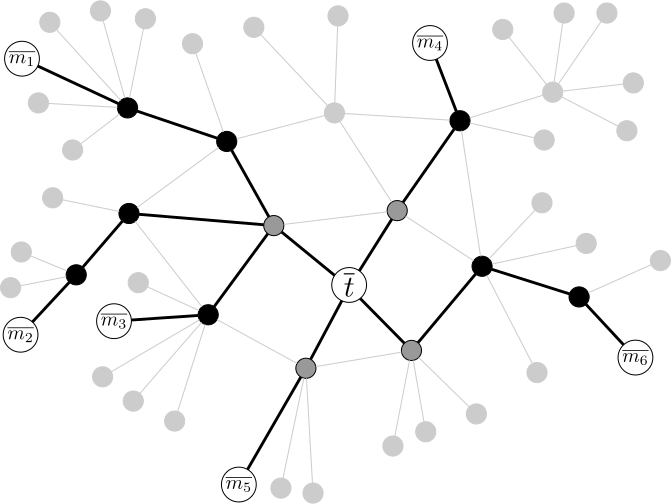
\includegraphics[width=0.83\columnwidth]{images/traceroute-many-to-one-target-core.png}}
\\
\subfloat{\includegraphics[width=0.83\columnwidth]{images/traceroute-many-to-one-target-border.png}}
\caption[Mesure de la liste des interfaces avec \traceroute]{Les liens en noir
sont parcourus par des sondes \traceroute, les liens en gris ne le sont pas. En haut (a):
la cible est dans le cœur et nous disposons d'un ensemble de moniteurs qui
permet d'observer au moins une fois chacun de ses voisins qui sont tous dans le
cœur égalemment. En bas (b): la cible est dans le cœur mais certains de ses
voisins sont dans le bord. Nous ne disposons pas de moniteurs dans les arbres
dont ces voisins sont les racines, donc nous n'observons que les voisins de la
cible qui sont dans le cœur.}
\label{fig:traceroute-many-to-one}
\end{figure}

\section{Estimation de la distribution de degré du cœur d'Internet au niveau
logique}
\label{sec:traceroute-many-to-many}

Nous avons expliqué dans les sections précédentes comment, à l'aide d'un
ensemble de moniteurs $M$ suffisamment grand et suffisamment bien réparti dans
le réseau, nous sommes capables d'observer des interfaces de tous les {\em
voisins dans le cœur} d'une cible $\overline{t}$ --- en particulier si cette
cible est dans le cœur, puisqu'une cible dans le bord possède au plus un unique
voisin tourné vers le cœur, \afortiori dans le cœur.

Remarquons d'abord que notre primitive de mesure de haut niveau permet d'obtenir
une {\em liste d'interfaces appartenant à des voisins dans le cœur d'une cible
désignée par l'une de ses interfaces}. Le problème de quotienter cette liste
pour identifier les interfaces appartenant à un même n\oe{}ud est le problème de
l'{\em anti-aliasing}, déjà évoqué précédemment. Des travaux
antérieurs~\cite{GunesS09,alias-bias,keys2010internet} ont déjà proposé des
solutions satisfaisantes pour résoudre ce problème et il sort donc du cadre de
ce travail.
Nous nous bornerons donc à mesurer de telles listes d'interfaces sans chercher
ici à réaliser l'{\em anti-aliasing}, c'est à dire passer de $M(t)$ à
$\overline{M(t)}$. Nous supposerons que cette partie du problème est acquise
comme résolue, et que si nous disposons de $M(t)$, alors nous pouvons
directement déduire $\overline{M(t)}$.

L'application de notre méthode {\em mesure orientée propriétée} aux {\em
routeurs du cœur de la topologie logique d'Internet} consiste à appliquer notre
{\em primitive de mesure de haut niveau basée sur \traceroute} depuis un
ensemble de moniteurs vers un certain ensemble de cibles $T$, {\em tiré de
manière uniformément aléatoire parmi les adresses du cœur de l'Internet} (c'est
à dire {\em sans biais de sélection}).
Commençons par définir notre méthode pour un certain ensemble de moniteurs vers
un ensemble cibles dans le cœur d'Internet:

\begin{definition}[Mesure depuis un ensemble de moniteurs d'un ensemble de
cibles] Soit $T = \{t_1, \ldots, t_n\} \subset \IPSet$ un ensemble de cibles
désignées par leurs interfaces tel que pour chaque $k$, $\overline{t_k} \in
C_3$.
On note $M(T) = \{(t_1, M(t_1)), \ldots, (t_n, M(t_n))\}$, et $\overline{M(T)} =
\{(\overline{t_1}, \overline{M(t_1)}, \ldots, (\overline{t_n},
\overline{M(t_n)})\}$. 
\end{definition}

On va en particulier s'intéresser à une propriété de $M(T)$, la distribution de
degré dans le cœur mesurée de notre ensemble de cibles:

\begin{definition}[Mesure depuis un ensemble de moniteurs de la distribution de
degré dans le cœur d'un ensemble de cibles]
Soit $T$ un ensemble de cibles et $M$ un ensemble de moniteurs. On note
$d(\overline{M(T)})$ la distribution des degrés mesurés, définie par
$d(\overline{M(T)})(k) = |\{ \overline{t}, |\overline{M(t)}| = k \}|$. On note
$\hat{d}(\overline{M(T)})$ cette distribution normalisée (telle que sa somme
soit égale à 1).
\end{definition}

Si les informations données par $M(T)$ sont intéressantes dans l'absolu, le
principe de {\em mesure orientée propriétée} repose sur notre capacité à déduire
des {\em propriétés de la topologie logique d'Internet} à partir de mesures
ciblées. Plus précisément, nous allons tenter d'estimer la distribution de degré
dans le cœur des n\oe{}uds du cœur, définie par:

\begin{definition}[Distribution de degré (dans le cœur) du cœur d'Internet]
On note $d(C_3)$ et on appelle {\em distribution de degré (dans le cœur) du
cœur d'Internet} la distribution définie par $d(C_3)(n) = |\{ \overline{v}
\in C_3, |C_3(V(\overline{v}))| = n \}|$. On note $\hat{d}(C_n)$ cette
distribution normalisée (telle que sa somme soit égale à 1).
\end{definition}

Notre objectif est, en ayant à notre disposition un ensemble de moniteurs $M$
qu'on suppose assez grand et assez bien distribué pour mesurer correctement
n'importe quelle cible $t$ donnée, de choisir un ensemble de cibles $T$ de telle
sorte que $\hat{d}(\overline{M(T)}) = \hat{d}(C_3)$, ou de minimiser autant que
possible la différence entre ces deux distributions (définie par $||
\hat{d}(\overline{M(T)} - \hat{d}(C_3)|| = \sum_{n}
|\hat{d}(\overline{M(t)})(n) - \hat{d}(C_3)(n)|$).
De cette manière, nous pouvons effectuer une mesure ciblée (de l'ensemble des
cibles $T$) afin d'estimer $\hat{d}(C_3)$, une propriété topologique
fondamentale de $G_3$. Pour ce faire, nous allons choisir $T$ de telle manière
qu'il soit un {\em échantillon représentatif} de $C_3$ du point de vue de
l'observation de cette propriété. Autrement formulé, supposons que $T$ soit un
ensemble de cibles tel que $\overline{T}$ soit un ensemble tiré de manière {\em
uniformément aléatoire} dans le cœur d'Internet. Alors les propriétés
topologiques des n\oe{}uds de $\overline{T}$ sont représentatives des propriétés
topologiques des n\oe{}uds de $C_3$, et en particulier, plus $\overline{T}$ est
grand (en restant uniformément aléatoire), plus les propriétés des n\oe{}uds de
$\overline{T}$ sont proches de celles de la totalité du cœur d'Internet. Pour le
cas de la distribution de degré, on peut le formaliser de la manière suivante:

\begin{proposition}[Estimation de la distribution de degré du cœur logique
d'Internet] Soit $M$ un ensemble de moniteurs suffisamment grand et suffisamment
bien réparti. Soit $(T_k)_k$ une suite d'ensembles de cibles telle que la suite
$(|\overline{T_k}|)_k$ soit strictement croissante et chaque $\overline{T_k}$
est un ensemble de cibles tiré de manière uniformément aléatoire dans $C_3$.
Alors la suite $(\varepsilon_k)_k = (||\hat{d}(\overline{M(T_k)}) -
\hat{d}(C_3)||)_k$ tend vers 0.
\label{prop:traceroute-estimation}
\end{proposition}

La qualité de l'estimation $(\varepsilon_k)$, si l'on suppose que chaque $(T_k)$
est un échantillon uniforme de taille $|T_k|$, n'est pas un problème
topologique, mais un problème statistique. On peut interpréter $\hat{d}(C_3)$
comme un ensemble de variables aléatoires $X_n = \hat{d}(C_3)(n)$ et chaque
$\hat{d}(\overline{M(T_k)})(n)$ comme un estimateur de $X_n$. Dans ce cas, on
peut tester l'adéquation empirique de $\hat{d}(\overline{M(T_k)})$ avec une
distribution donnée, par exemple une loi de Poisson ou une loi de puissance, en
réalisant des tests d'hypothèses classiques. Ces tests sortent du strict cadre
de notre travail, mais on peut mentionner le {\em test du $\chi^2$}, ou le {\em
test de Kolmogorov-Smirnov}~\cite{stephens1979tests}.

Cela signifie que pour obtenir une estimation aussi précise que l'on souhaite de
la propriété qui nous intéresse, la distribution de degré du cœur logique
d'Internet (et la comparer à une distribution théorique donnée), il suffit de
réaliser les conditions suivantes :
\begin{bulletpoints}
  \item (1) Être capable de tirer un ensemble de cibles $T$ d'interfaces de
  n\oe{}uds du cœur tel que $\overline{T}$ soit uniformément aléatoire dans $C_3$ et
  suffisamment grand,
  \item (2) Disposer d'un ensemble de moniteurs $M$ suffisamment grand et
  suffisamment bien réparti,
  \item (3) Effectuer une mesure correcte de $M(T)$, ce qui suppose en
  particulier d'éliminer les $m(t)$ incorrects (les couples $(m, t)$ tels que les
  routes de $m$ vers $t$ ne sont pas toutes de même longueur, ou tels que $m$
  soit un descendant de l'arbre enraciné de racine $t$),
  \item (4) Calculer $\overline{M(T)}$ (pour déduire
  $\hat{d}(\overline{M(T)})$).
\end{bulletpoints}

Nous examinerons la condition (1) dans la~\refsec{traceroute-sampling}. La
condition (2) sera supposée vraie, mais le réalisme de cette hypothèse sera
examiné à travers des simulations en~\refsec{traceroute-simuls}. La condition
(3) repose sur un filtrage rigoureux des données collectées par \traceroute
\aposteriori que nous allons décrire en ~\refsec{traceroute-filtering}. Enfin,
la condition (4) repose sur des méthodes d'{\em anti-aliasing} décrites dans des
travaux antérieurs.

\section{\'Echantillonage des cibles dans le cœur}
\label{sec:traceroute-sampling}

Dans la~\refsec{traceroute-many-to-many}, nous avons montré que notre méthode
orientée propriété pour estimer la distribution de degré du cœur logique
d'Internet repose sur notre capacité à sélectionner un ensemble de cibles $T$
tel que $\overline{T}$ soit uniformément aléatoire dans le cœur d'Internet. Dans
le strict cadre de notre travail sur la topologie logique, nous n'avions pas
réussi à aller jusqu'au bout de cette démarche\footnote{Même si nous y sommes
parvenus dans des travaux ultérieurs (\refchap{udpping})}. Nous avons cependant
mis au point une méthode de sélection qui permet de sélectionner $T$ tel que $T$ soit
{\em uniformément aléatoire dans l'ensemble des interfaces appartenant à des
n\oe{}uds du cœur}. Nous procédons en plusieurs étapes, en supposant que l'on
dispose d'un ensemble $M$ de moniteurs suffisamment grand et suffisamment bien
réparti:
\begin{bulletpoints}
  \item (1) On tire {\bf de manière uniformément aléatoire} un ensemble $T_0$
  d'entiers 32 bits, qui représentent des {\em adresses \ip} (qui peuvent être
  valides ou invalides),
  \item (2) On extrait l'ensemble $T_1 = T_0 \cap \IPSet$ de ces adresses qui
  sont valides,
  \item (3) On utilise notre primitive de mesure de haut niveau pour calculer
  $M_1 = M(T_1)$,
  \item (4) On extrait de cette mesure $M_1$ le sous-ensemble de données $M_2$
  dont on a supprimé les données incorrectes, c'est à dire issues de couples $(m, t)$
  tels qu'il existe des routes de longueurs différentes de $m$ vers $t$ ou tels
  que $m$ soit un descendant de $t$ dans $A(\overline{t})$,
  (\cf~\refsec{traceroute-filtering})
  \item (5) On extrait de $T_1$ le sous-ensemble $T_2$ des cibles $t$ telles que
  $M_2(t) = M(t) \cap M_2$ observe $\overline{t}$ avec un degré tourné vers le
  cœur {\bf strictement supérieur} à 1.
\end{bulletpoints}

Notons d'abord qu'aucune de ces étapes ne nuit à l'uniformité aléatoire de
l'ensemble des cibles, et que par conséquent l'ensemble final $T_2$ est
également uniformément aléatoire. Il nous reste à vérifier que $T_2$ est bien un
sous-ensemble de $C_3$. Les étapes (2), (3) et (4) garantissent, comme démontré
lors des sections précédentes, que $M_2(t)$ correspond bien à un ensemble
d'interfaces des voisins tournés vers le cœur de $\overline{t}$. Comme $M$ est
supposé suffisamment grand et suffisamment bien réparti, alors $M_2(t)$ contient
au moins une interface de chacun des voisins tournés vers le cœur de
$\overline{t}$. En appliquant une méthode d'{\em anti-aliasing} à $M_2(t)$, on
obtient $\overline{M_2(t)}$ et donc $|\overline{M_2(t)}|$, le {\em degré dans le
cœur} de $\overline{t}$, c'est à dire le nombre de voisins {\em tournés vers le
cœur} de $\overline{t}$. L'étape (5) revient donc à conserver uniquement les
cibles qui ont {\em au moins 2} voisins {\em tournés vers le cœur}. Or, par
construction, les n\oe{}uds du bord sont {\bf exactement} les n\oe{}uds qui ont 0 ou 1
seul voisin {\em tourné vers le cœur}, puisqu'ils sont situés sur des arbres;
réciproquement, si un n\oe{}ud est sur un arbre, alors il est sur le bord
(\reffig{traceroute-core-degree-1}). On peut en conclure que $\overline{T_2}
\subset C_3$, ce que nous cherchions à démontrer.

\realfig{traceroute-core-degree-1.png}{Sélection des cibles du cœur par leur
degré dans le cœur mesuré avec \traceroute} {On étiquette les n\oe{}uds de $G_3$ par leur degré mesuré depuis
l'ensemble $M$. Les n\oe{}uds de $C_3$ (en gris) sont les n\oe{}uds dont le degré
mesuré est strictement supérieur à 1 qui ne sont pas des ancêtres des moniteurs
dans le sous-arbre qui les relie au c\oe{}ur (en rouge).}
{traceroute-core-degree-1}

\section{Filtrage des résultats}
\label{sec:traceroute-filtering}

La méthode que nous avons décrite en~\refsec{traceroute-many-to-many}, et en
particulier l'échantillonage des cibles dans le cœur
détaillé en \refsec{traceroute-sampling}, repose sur deux hypothèses. Pour une
certaine mesure $M(T)$, composée de mesures ponctuelles $m(t)$, nous supposons que (1)
les chemins empruntés par \traceroute depuis $m$ vers $t$ sont de longueur
constante, et que (2) $m$ n'est pas dans $A(\overline{t})$. Pour
garantir ces deux hypothèses, nous partons d'une mesure $M(T)$ et nous détectons
les couples $(m, t)$ qui ne satisfont pas soit (1) soit (2); nous extrayons un
sous-ensemble des données privé de ces couples. Il nous suffit donc de disposer
d'un moyen de tester (1) et (2) pour chaque couple $(m, t) \in M \times T$.

Le cas (1) peut être détecté en exécutant plusieurs fois \traceroute depuis $m$
vers $t$ successivement. En effet, \traceroute, dans l'interprétation rigoureuse
que nous en avant donné en~\refsec{traceroute-rigor}, fournit une information
sur la longueur de la route empruntée par la dernière sonde, celle qui atteint
la cible $\overline{t}$. En répétant plusieurs fois \traceroute, on peut en
principe détecter, en comparant les longueurs obtenues, la propriété désirée. Si
lors des mesures successives, \traceroute renvoie au moins deux longueurs
distinctes, alors on peut supprimer le couple $(m, t)$ de notre jeu de données
en le considérant comme suspect et potentiellement tel que $\overline{m(t)}$ ne
soit pas un voisin de $\overline{t}$. Idéalement, il nous faudrait être capable
de majorer le risque, c'est à dire d'obtenir une majoration de la probabilité
qu'il existe bien des routes de $m$ vers $t$ de longueur différentes, en
supposant que la réalisation de \traceroute depuis $m$ vers $t$ au cours de $n$
itérations ont toutes fourni une longueur égale.

Nous n'avons pas pu obtenir de réponse dans le cas général, mais nous avons
étudié un cas simple pour comprendre le phénomène. Supposons qu'il y ait
exactement deux routes de $m$ vers $t$ de deux longueurs distinctes $l_1 < l_2$,
qui sont équiprobables, c'est à dire que pour chaque \traceroute de $m$ vers
$t$, ces deux routes soient empruntées par la dernière sonde (celle qui atteint
$\overline{t}$) avec une probabilité de $\frac{1}{2}$. Quand une sonde
\traceroute est envoyée depuis $m$ vers $t$ avec un \ttl égal à $l_1$,
elle emprunte l'une de ces deux routes. Si elle emprunte la route la plus courte
(de longueur $l_1$), alors cette sonde atteint $\overline{t}$ et \traceroute se
termine et renvoie cette longueur $l_1$. Si au contraire elle emprunte la route
la plus longue (de longueur $l_2$), alors \traceroute se terminera
ultérieurement et renverra une longueur entre $l_1 + 1$ et $l_2$. Il s'ensuit
que, si l'on effectue \traceroute depuis $m$ vers $t$, la probabilité que l'on observe {\em
toujours} la longueur $l_1$ est majorée par $\frac{1}{2^{n-1}}$. Au moins dans
ce cas simplifié, le risque de ne pas rejeter $(m, t)$ alors qu'il est possible
que $\overline{m(t)} \notin V(\overline{t})$ décroît exponentiellement avec le
nombre de fois qu'on exécute \traceroute sans constater de longueurs distinctes.
On peut donc raisonnablement supposer qu'il suffit de seulement quelques
exécutions successives de \traceroute depuis $m$ vers $t$ (de l'ordre d'une
dizaine) pour garantir avec une très grande confiance que $\overline{m(t)} \in
V(\overline{t})$. On peut augmenter arbitrairement la confiance dans cette
garantie en augmentant le nombre d'itérations de \traceroute. Une autre méthode,
la {\em méthode des routes longues}, est une autre perspective qui sera discutée
plus loin (\refchap{conclusion}).

Le cas (2) peut également être résolu en utilisant des mesures \traceroute
complémentaires. Par définition, il ne peut se produire que dans le cas où
$\overline{m}$ est un n\oe{}ud du bord, et un descendant de $A(\overline{t})$.
Donc $\overline{t}$ sépare $V_3$ en deux parties $A = A(\overline{t})$ et
$\complement_A = V_3 \setminus A(\overline{t})$, telles que tous les chemins
depuis un n\oe{}ud de l'une de ces parties vers un n\oe{}ud dans l'autre de ces
parties passe nécessairement par $\overline{t}$
(\reffig{traceroute-detection-sousarbre}).
On veut être capable de détecter le cas où $m \in \complement_A$. On effectue
alors, pour chaque couple de moniteurs $(m_1, m_2)$, \traceroute depuis $m_1$
vers $m_2$. Comme $\overline{t}$ répond aux sondes \traceroute (sinon il ne
serait pas dans $T$), alors si $m_1$ et $m_2$ ne sont pas dans la même partie du
découpage entre $A$ et $\complement_A$, alors une interface de $\overline{t}$
(détectée comme telle par {\em anti-aliasing}) est nécessairement présente dans
la sortie de \traceroute de $m_1$ vers $m_2$, qu'on notera $\overline{[m_1,
m_2]}$.
Par contraposée, si $\overline{t}$ n'{\em apparaît pas} dans \traceroute depuis
$m_1$ vers $m_2$, c'est à dire si $\overline{t} \notin \overline{[m_1, m_2]}$,
alors nécessairement soit $m_1$ et $m_2$ sont tous les deux dans $A$, soit ils
sont tous les deux dans $\complement_A$.

\realfig{traceroute-detection-sousarbre.png}{Découpage de $G_3$ par rapport à
une cible} {$\overline{t}$ est un n\oe{}ud du bord, et donc racine d'un arbre
$A$. On découpe $G_3$ en deux parties $A$ et $\complement_A$. Tous les chemins
qui passent de $A$ à $\complement_A$ passent par $\overline{t}$ et
réciproquement.
On peut donc déduire que si deux moniteurs sont chacun dans une partie
différente de $G_3$, alors $\overline{t}$ apparaît dans \traceroute depuis l'un
des moniteurs vers l'autre.} {traceroute-detection-sousarbre}

Fixons à présent un moniteur $m$ pour déterminer s'il se trouve dans le cas (2).
Supposons que c'est le cas et que $m \in A$. Alors tous les moniteurs dans  $M
\cap \complement_A$ sont tels que $\overline{t}$ apparaît dans \traceroute vers
$m$. Comme par hypothèse $M$ est suffisamment grand et suffisamment bien réparti
pour observer correctement le cœur d'Internet, il n'est pas vraissemblable que
presque tous les moniteurs se trouvent dans A. Donc $M \cap \complement_A$
représente nécessairement une forte proportion des moniteurs, qu'on peut minorer
par exemple à $p = \frac{1}{2}$. Alors nécessairement au moins une proportion
$p$ des sorties de \traceroute depuis $M$ vers $m$ contiennent $\overline{t}$.
Par contraposée, si moins d'une proportion inférieure à $p$ des sorties de
\traceroute depuis $M$ vers $m$ contiennent $\overline{t}$, alors on peut {\bf
déduire} que $m \notin A$. Pour résoudre le cas (2), on compte donc le nombre
d'occurences parmis les sorties de \traceroute depuis $M$ vers $m$ et on
supprime $(m, t)$ de notre jeu de données si $\overline{t}$ apparaît dans au
moins une proportion $p$ des résultats. On ne peut pas conclure la réciproque,
mais nous nous satisfaisons du risque de faux-positifs (éliminer $(m, t)$ alors
que $m \notin A(t)$), notre considération essentielle étant d'avoir le plus
faible taux de faux-négatif (conserver $(m, t)$ alors que $m \in A(t)$). Notons
que l'estimation $p = \frac{1}{2}$ est {\em très} prudente, en pratique nous
avons grossièrement estimé que $p$ est au moins de $\frac{9}{10}$ si l'ensemble
$M$ est bien choisi.

En résumé, pour filtrer les résultats et garantir que $\overline{M(T)}$
correspond bien à l'observations de voisins des cibles $\overline{T}$ qui sont
tournées vers le cœur, nous procédons de la manière suivante :
\begin{bulletpoints}
\item Pour chaque couple $(m, t)$ on effectue \traceroute $n$ fois depuis $m$
vers $t$ et on supprime $(m, t)$ de notre jeu de données si on obtient au moins
2 longueurs distinctes. (Traitement du cas (1))
\item Pour chaque couple $(m_1, m_2)$ on effectue \traceroute depuis $m_1$ vers
$m_2$ et pour chaque $m \in M$ et chaque $t \in \overline{t}$ on compte $N(m,
\overline{t})$ le nombre de moniteurs $m'$ tels que $\overline{t}$ apparaît dans \traceroute depuis $m'$
vers $m$. Si $\frac{N(m, \overline{t})}{|M|} > p = \frac{1}{2}$ alors on
supprime $(m, t)$ de notre jeu de données. (Traitement du cas (2))
\end{bulletpoints}

\section{Simulations}
\label{sec:traceroute-simuls}

La qualité de notre estimation de la distribution de degré dans le cœur des
routeurs du cœur d'Internet repose sur une hypothèse importante: que l'on
dispose d'un ensemble de moniteurs $M$ qui soit suffisamment grand et
suffisamment bien réparti. Dans cette section, nous ne cherchons pas à
déterminer si un ensemble $M$ {\em donné} souscrit à ces hypothèses (nous
reviendrons sur cette question dans le~\refchap{udpping} et
le~\refchap{revtables}), mais plutôt à déterminer s'il est {\em réaliste} de
supposer qu'avec un ensemble limité de moniteurs, on peut correctement estimer
le degré dans le cœur d'une cible, et a fortiori la distribution de degré dans
le cœur du cœur d'Internet. Pour ce faire, nous avons réalisé des simulations de
notre méthode de mesure sur des modèles simplifiés d'Internet inspirés des
approches historiques.

Notre première hypothèse simplificatrice, correspondant aux approches
historiques de modélisation~\cite{LakhinaBCX03,GuillaumeLM06} et
d'observation~\cite{GuillaumeLM06}, est que les sondes empruntées par
\traceroute suivent des plus courts chemins (choisis aléatoirement, lorsque
plusieurs sont disponibles) pour atteindre leur destination. Il est à noter que
cette hypothèse n'est pas celle que nous avons refuté
en~\refsec{traceroute-rigor}, puisqu'elle porte sur chacune des sondes de
\traceroute, pas sur la sortie de \traceroute. L'ensemble des moniteurs $M$ est
un ensemble uniformément aléatoire dans le graphe et l'ensemble des cibles $T$
est la totalité du graphe.

Notre deuxième hypothèse simplificatrice concerne le type de topologie sur
lequel nous réalisons nos simulations. Nous avons utilisé dans le cadre de ce
travail des graphes aléatoires à distribution de degré suivant une loi de
Poisson. Nous montrerons que nous avons ultérieurement réalisé des simulations
sur d'autres topologies dans le cadre de notre travail sur la topologie physique
(\refchap{udpping}). Un graphe aléatoire en loi de Poisson possède deux
paramètres principaux: le nombre de n\oe{}uds et son degré moyen. Il est
difficile en pratique de simuler des graphes dont la taille totale est comparable à celle
d'Internet (qui se compte en milliards de n\oe{}uds), nous avons donc choisi
d'utiliser des graphes de taille $10^6$ et $10^7$. Pour le degré moyen, nous
avons choisi un degré moyen de 20, ce qui est élevé par rapport aux
hypothèses des approches historiques, et \apriori défavorable à notre méthode
(qui par nature est plus efficace en principe lorsque le degré des cibles est
faible et requiert donc moins de moniteurs). Nous avons constaté que les
résultats obtenus pour des degrés moyens inférieurs étaient qualitivement
identiques au cas où le degré moyen est 20.

Des simulations comparables ont été réalisées par Lakhina \etal
\cite{LakhinaBCX03} pour évaluer les résultats de l'évaluation de la
distribution de degré d'un graphe en utilisant la méthode classique consistant à
aggréger les plus courts chemins entre un ensemble de 10 moniteurs et un
ensemble de $10^3$ cibles. Dans ces simulations, les graphes étaient également
des graphes aléatoires en loi de Poisson, de taille $10^5$ et de degré moyen 15.
L'un des résultats les plus édifiants de ces simulations est que la distribution
alors mesurée n'est pas une loi de Poisson, mais ressemble davantage à une loi
de puissance ({\em powerlaw}). Ce résultat a même été démontré formellement dans
le cas d'un seul moniteur~\cite{AchlioptasCKM09}. À défaut d'invalider
totalement la méthode classique, ces simulations montrent la pertinence de la
démarche: même sur des graphes simulés, l'approche historique est
intrinsèquement biaisée. Si notre méthode donne de meilleurs résultats dans des
conditions similaires, on peut raisonnablement espérer qu'elle donnera également
des meilleurs résultats lors d'une mesure réelle.

Nous avons donc calculé les distributions mesurées par notre méthode sur ces
graphes artificiels (\reffig{traceroute-simuls}). Comme on pouvait s'y attendre,
lorsque le nombre de moniteurs est très faible ($|M| = 25$), le degré moyen
observé est 15. Ce n'est pas surprenant puisque le nombre de moniteurs est très
proche du degré moyen réel, et que donc les n\oe{}uds de fort degré ($> 25$) ne
peuvent pas être correctement observés. Il est toutefois intéressant de
remarquer que même dans ce cas très défavorable, la {\em nature} de la
distribution est correctement observée, puisqu'on observe une distribution en
loi de Poisson, et seul son paramètre (le degré moyen) est sous-évalué, là où la
méthode classique observe une distribution de nature différente (loi de
puissance)\footnote{Voir \cite{LakhinaBCX03}.}.

\realfig{traceroute-simuls.png}{Simulation de la topologie logique} {Pour chacun
des graphes (de taille $10^6$ (gauche) et $10^7$ (droite)) on compare la distribution de degré réelle
({\em full.out}) avec la distribution de degré mesurée avec différents ensemble
de moniteurs, de taile 25, 100, 200, et 500. La nature de la distribution est toujours bien
observée comme une loi de Poisson. À partir de 200 moniteurs, et indépendamment
de la taille du graphe, la distribution réelle et la distribution mesurée sont
presque indiscernables, même pour les forts degrés.} {traceroute-simuls}

En augmentant le nombre de moniteurs, la qualité de l'estimation s'améliore très
rapidement. À partir de $|M| = 200$, la distribution observée est indiscernable
de la distribution réelle, et il n'y a plus d'amélioration significative en
augmentant ce nombre. On remarque en particulier que même pour les cibles de
très fort degré ($> 30$), l'estimation est excellente. Pour les deux graphes (de
taille $10^6$ et de taille $10^7$), le degré maximal observé n'est inférieur que
de deux unités au degré maximal réel (43 au lieu de 45 et 46 au lieu de 48).
Les n\oe{}uds de degré réel $>30$ sont observés pour 97\% d'entre eux comme ayant
un degré $>30$ (89\% pour les n\oe{}uds de degré $>35$), ce qui signifie que les
n\oe{}uds de fort degré ne sont pas observés avec un degré relativement faible.
Nous pouvons donc conclure qu'au moins sur de tels graphes, avoir un ensemble
moniteurs répartis aléatoirement de taille modeste ($|M| = 200$, ce qui est
comparable à la taille de l'ensemble des moniteurs \planetlab) suffit à très
bien estimer la distribution de degré.

Cependant, $V_3$ est \apriori beaucoup plus vaste, puisque le nombre d'hôtes
connectés est plus proche de $10^9$ en ordre de
grandeur~\cite{consotium2010isc}. Mais dans nos simulations, on ne constate
aucune différence notable entre les résultats obtenus pour le graphe de
taille $10^6$ et pour le graphe de taile $10^7$. En particulier, le nombre de
moniteurs requis pour réaliser une observation de qualité, à part pour certains
n\oe{}uds de degré extrêmement élevé, apparaît indépendant de la taille du graphe.
Ceci suggère que les résultats devraient être de la même qualité pour des
graphes arbitrairement grand, sans qu'il soit nécessaire d'augmenter le nombre
de moniteurs en conséquence. Nous n'avons pas pu réaliser la preuve formelle de
cette hypothèse, mais nous l'avons ultérieurement éprouvée pour d'autres
topologies (\refchap{udpping}).

\section{Mesure avec \planetlab}
\label{sec:traceroute-measurement}

Afin d'attester la faisabilité pratique de la mesure réalisée par $M(T)$ pour un
certain ensemble $M$ de moniteurs et un échantillon $T$ de cibles, nous
avons implémenté une mesure réelle. Cette mesure n'avait pas pour objectif d'estimer
directement la distribution $\hat{d}(V_3)$ mais plutôt d'explorer les problèmes
pratiques rencontrés lors d'une mesure et d'y chercher des solutions.

Pour cette mesure, nous avons utilisé un ensemble de moniteurs dans l'ensemble
des machines mises à notre disposition par \planetlab~\cite{planetlab}.
L'évaluation de la qualité de cet ensemble de moniteurs a fait l'objet d'un
travail plus approfondi au~\refchap{udpping}, en particulier pour déterminer si
cet ensemble est bien "suffisamment grand et suffisamment réparti", tel que nous
l'avons défini dans ce chapitre. Certains de ces moniteurs sont sujets à des
problèmes techniques réguliers (coupures de courant, déconnexions intempestives,
filtrage d'\icmp, \ldots). Comme il est difficile de détecter ces problèmes
\apriori, nous avons décidé d'utiliser {\em tous} les moniteurs à notre
disposition et de procéder à un nettoyage des données \aposteriori, une étape de
toutes manières imposée par la méthode théorique que nous avons décrite
en~\refsec{traceroute-sampling} et ~\refsec{traceroute-filtering}.

De manière analogue, nous avons tiré un échantillon aléatoire d'entiers 32 bits,
que nous avons expurgé de ceux correspondant à des adresses \ip invalides pour
obtenir une liste d'adresses \ip valides. Nous avons envoyé une sonde \icmp~{\sc
Echo Request} à chacun de ces adresses et enregistré les $10^4$ premières à
répondre.

Munis de cette liste, nous avons effectué une collecte de données sur environ
30h de la manière suivante. Pour chaque moniteur à notre disposition, nous avons
généré une permutation aléatoire de la liste des cibles, et lancé \traceroute
depuis ce moniteur vers chacune des cibles dans l'ordre de cette permutation
de la liste. Nous utilisons ici \traceroute~\icmp, ce qui signifie que les
sondes envoyées contiennent le message \icmp~{\sc Echo Request}, auquel les
cibles devraient en principe répondre puisqu'elles ont été sélectionnées au
départ avec ce message. Cette opération a été répétée 10 fois depuis chaque
moniteur, et toutes les sorties de \traceroute ont été archivées pour analyse
ultrérieure. Les moniteurs n'ayant toujours pas terminé leur mesure à l'issue de
ces 30h (moins de 10\% des moniteurs qui avaient démarré), pour des raisons
diverses (coupures, problèmes de réseau,~\ldots), ont été supprimés du jeu de
données.

La première étape d'analyse a consisté à supprimer de notre jeu de données les
moniteurs et les cibles considérées comme peu fiables. Un des points
méthodologiquement important est que les critères utilisés pour supprimer une
cible de notre jeu de données doivent être indépendants \apriori du degré de
cette cible; dans le cas contraire, ce filtrage pourrait biaiser la distribution issue
de la mesure. En n'utilisant uniquement que des critères de filtrages \apriori
indépendants du degré, nous nous assurons que nous n'induisons pas un biais
méthodologique. Notre premier filtrage permet d'éliminer de notre jeu de données
les moniteurs et les cibles qui ont été temporairement indisponibles pendant
notre mesure. Pour ce faire, on compte pour chaque moniteur et pour chaque cible
le nombre de sondes \traceroute qui ont atteint leur destination (depuis un
moniteur ou vers une cible).

\realfig{traceroute-coupure-moniteurs.png}{Répartition des \traceroute par
moniteur} {Pour chaque moniteur, on compte le nombre de \traceroute qui ont atteint leur
cible. Un point $(x, y)$ de la distribution cumulative montrée ici se lit: {\em
$x$ moniteurs ont moins de $y$ \traceroute ayant atteint leur cible}. En
particulier, le point $(68, 71783)$ indique qu'au plus 68 moniteurs ont moins de
71783 \traceroute ayant atteint leur cible.}{traceroute-coupure-moniteurs}

\realfig{traceroute-coupure-cibles.png}{Répartition des \traceroute par cible}
{Pour chaque cible, on compte le nombre de \traceroute qui ont atteint leur
cible. Un point $(x, y)$ de la distribution cumulative montrée ici se lit: {\em
$x$ cibles ont moins de $y$ \traceroute les ayant atteint}. En particulier, le
point (2314, 3502) indique qu'au plus 2314 cibles ont moins de 3502 \traceroute
les ayant atteint.}{traceroute-coupure-cibles}

Au total, nous avons collecté 36,928,702 sorties de \traceroute depuis 544
moniteurs vers 10,000 cibles, et examiné leur répartition parmi les moniteurs
(\reffig{traceroute-coupure-moniteurs}) dont elles étaient à l'origine et les
cibles (\reffig{traceroute-coupure-cibles}) dont elles étaient la destination.
Nous avons compté pour chaque moniteur le nombre de \traceroute ayant
atteint leur cible. Nous avons constaté que seuls 68 moniteurs sur 544 (environ
12\%) comptaient moins de 71783 \traceroute ayant atteint leur cible, tandis que
le moniteur ayant le {\em plus} de \traceroute ayant atteint leur cible en
compte 77,316 (environ 92\%). Nous avons donc conservé 88\% de notre ensemble
initial de moniteurs, qui observent {\em tous} au moins 92\% autant de
\traceroute que le {\em meilleur} moniteur du point de vue de ce critère. De
manière analogue, nous avons compté pour chaque cible le nombre de \traceroute
l'ayant atteinte. Il est important de rappeler qu'\apriori, ce nombre n'a aucune
corrélation avec le degré du n\oe{}ud \LLL sous-jacent. Nous avons constaté que
2,314 cibles sur les 9,395 qui ont été atteintes par au moins un \traceroute
(environ 25\%) ont été observées par moins de 3,502 \traceroute, à comparer aux
4,760 \traceroute ayant atteint la cible qui l'a été le plus (environ 74\%).
Nous avons donc conservé 7,081 cibles ayant chacune été observée par au moins 3,502
\traceroute ayant atteint leur cible. Remarquons que comme chaque moniteur
génère au plus 10 sorties de \traceroute différentes, chacune de ces cibles a
donc été observée par au moins 350 moniteurs.

Avec cette expérimentation, nous avons aussi pu attester de la pertinence de
notre méthode de détection des cas où certains moniteurs ont des routes de
différentes longueurs vers certaines cibles. Plus précisément, rappelons qu'un
couple $(m, t)$ est considéré comme impropre et éliminé de notre jeu de données
si, au cours des 10 \traceroute depuis $m$ vers $t$, au moins 2 longueurs
différentes ont été observées. Environ 75\% de ces couples ont produit des
résultats de \traceroute de longueurs constantes. Seulement 980 cibles sur les
7,081 restantes à ce stade (environ 14\%) sont observées par moins de 350
moniteurs avec des \traceroute de longueur constante
(\reffig{traceroute-coupure-suspects}). Inversement, toutes les cibles restantes
ont été observées par {\em au moins} 350 moniteurs avec tous leurs \traceroute à
longueur constante, suggérant que pour les couples $(m, t)$ restants, $m(t)$ est
bien une interface d'un voisin de $\overline{t}$. Après suppression de ces
couples impropres, il restait 6,101 cibles.

\realfig{traceroute-coupure-suspects.png}{Cibles atteintes par des moniteurs de
longueur constante} {Pour chaque cible, on compte le nombre de moniteurs dont
{\em tous} les résultats de \traceroute vers cette cible ont donné la même
longueur. Un point $(x, y)$ de la distribution cumulative montrée ici se lit: au
plus $y$ cibles ont été observées par moins de $x$ moniteurs avec uniquement des
résultats de même longueur. En particulier, le point $(350, 980)$ indique qu'au
plus 980 cibles ont été observées par moins de 350 moniteurs avec des résultats
de même longueur.}{traceroute-coupure-suspects}

Au cours de cette mesure d'expérimentation nous n'avons pas obtenu d'estimation
directe de la distribution de degré. Plusieurs étapes intermédiaires auraient
encore été nécessaires, telles que nous les décrirons
en~\refsec{traceroute-protocol}. Nous avons toutefois, comme illustration du
principe, calculé la distribution du {\em nombre d'interfaces tournées vers le
cœur de voisins tournés vers le c\oe{}ur} de notre ensemble de cibles (dont nous
n'avons pas vérifié à ce stade qu'elles sont elles-mêmes dans le c\oe{}ur)
({\reffig{traceroute-distrib}}).

\realfig{traceroute-distrib.png}{Distribution du nombre d'interfaces tournées
vers le c\oe{}ur des voisins tournés vers le c\oe{}ur de notre ensemble de cibles} {Distribution du nombre
d'interfaces tournées vers le c\oe{}ur des voisins tournés vers le c\oe{}ur de notre
ensemble de cibles. Un point $(x, y)$ dans cette distribution signifie que $y$
cibles ont été observées avec $x$ interfaces tournées vers le c\oe{}ur de voisins
tournés vers le c\oe{}ur.} {traceroute-distrib}

\section{Protocole complet}
\label{sec:traceroute-protocol}

Après avoir étudié les aspects à la fois théoriques et pratiques liés à notre
méthode de mesure, nous avons pu établir un protocole complet qui permet
d'évaluer la distribution de degré des routeurs du c\oe{}ur au niveau logique.

Soit les paramètres suivants :
\begin{itemize}
  \item $M_0$, un ensemble de moniteurs.
  \item $N \in \mathbb{N}$, un nombre initial de cibles.
  \item $n \in \mathbb{N}$, un nombre d'itération de \traceroute depuis chaque
  moniteur vers chaque cible.
  \item $p \in [0, 1]$, un seuil de rejet des moniteurs (tel que décrit en
  \refsec{traceroute-filtering}).
\end{itemize}

\begin{enumerate}
\item Pour chaque couple $(m, m')$ de moniteurs on effectue \traceroute depuis
$m$ vers $m'$ et on note $[m, m']$ la liste des adresses apparaissant dans la
sortie.
\item Pour chaque couple $(m, m')$ de moniteurs on effectue un {\em
anti-aliasing} sur chaque adresse dans $[m, m']$ et on obtient $\overline{[m,
m']} = \{ \overline{v}, v \in [m, m'] \}$.
\item On tire des entiers avec un générateur aléatoire uniforme dans $\IPSet$.
On envoie un paquet \icmp~{\sc Echo Request} aux adresses correspondantes, et on
accepte une adresse si on obtient une réponse \icmp~{\sc Echo Reply} adéquate.
On s'arrête lorsque $N$ réponses ont été acceptées, et on note $T_0$ l'ensemble
des adresses correspondantes ($|T_0| = N$).
\item Chaque moniteur $m \in M_0$ répète $n$ fois l'opération:
	\begin{itemize}
	  \item (4.a) Mélanger l'ensemble $T_0$ pour produire la liste $T_{m,n}$
	  \item (4.b) Pour chaque $t \in T_{m,n}$, effectuer \traceroute depuis $m$
	  vers $t$; on note la réponse de l'avant-dernière sonde $m_n(t)$ et $l_n(m, t)$ la
	  longueur du résultat, lorsque ces informations sont disponibles.
	\end{itemize}
On note $\hat{m}(t) = \cup_{n} \{ m_n(t) \}$ pour chaque $n$ où $m_n(t)$ est
défini (la $n$-ième itération de \traceroute depuis $m$ vers $t$ a obtenu une
réponse), et $\hat{m}(t) = \emptyset$ si aucun $m_n(t)$ n'est défini.
\item On supprime des données restantes tous les couples $(m, t)$ tel qu'il
existe $i,k$ tels que $l_i(m, t) \neq l_j(m, t)$.
\item On supprime des données collectées les moniteurs ayant un nombre
anormalement bas de réponses (au sens de la distribution cumulative) à leurs
sondes \traceroute.
\item On supprime des données restantes les cibles ayant un nombre anormalement
bas de réponses (au sens de la distribution cumulative) à leurs sondes
\traceroute.
\item On supprime des données restantes les cibles $t$ telles qu'il
existe au moins un moniteur $m$ tel qu'au moins une proportion supérieure à $p$ des autres
moniteurs $m'$ sont tels que $\overline{t} \in \overline{[m, m']}$ (indiquant
que $m$ est un descendant de $\overline{t}$ et donc que $\overline{t}$ est
possiblement dans le c\oe{}ur).
\item On note $M$ et $T$ les ensembles de moniteurs et de cibles après filtrage.
Pour chaque couple $(m, t)$ dans les données restantes, on effectue un
anti-aliasing de $\hat{m}(t)$ pour obtenir $\overline{\hat{m}(t)}
= \{ \overline{v}, v \in \hat{m}(t) \}$.
\item On estime alors que pour chaque $t \in T$, $V_{C_3}(\overline{t}) =
\cup_{m \in M} \overline{\hat{m}(t)}$. En particulier, on estime que
$d_{C_3}(\overline{t}) = |\cup_{m \in M} \overline{\hat{m}(t)}|$.
\item On calcule la distribution $d_{M,T}$ définie par $d_{M,T}(k) = |\{
\overline{t}, t \in T~et~d_{C_3}(\overline{t}) = k \}|$.
\item On en déduit la distribution normalisée $\hat{d}_{M,T}$ , une estimation
de la distribution de degré des routeurs du c\oe{}ur.
\end{enumerate}

On peut exprimer la "complexité" du protocole en termes de nombre de \traceroute
effectués au total et en nombre de requêtes d'anti-aliasing (qu'on considère
ici comme une opération atomique). On supposera que la longueur moyenne des
routes empruntées par \traceroute d'un moniteur à un autre est $\lambda$, et on
note $\tilde{d}$ le degré moyen de $T$.

\begin{bulletpoints}
\item {\bf Nombre de \traceroute effectués :} $O(|M_0|^2)$ pour l'étape (1),
$O(n)$ pour l'étape (4.b) répétée $N$ fois donc $O(n N)$ pour l'étape (4), soit
un total de \boldmath$O(|M_0|^2 + n N)$\unboldmath.
\item {\bf Nombre d'{\em anti-aliasing} effectués :} $O(\lambda|M_0|^2)$ pour
l'étape (2),  $O(\tilde{d} |M_0|)$ pour l'étape (5), soit un total
de \boldmath$O(\lambda |M_0|^2 + \tilde{d} |M_0|)$\unboldmath.
\end{bulletpoints}


On peut considérer que $\lambda$ peut être majoré par 20 (une estimation plus
fine de $\lambda$ peut être réalisée pour $M_0$ donné, lors de l'étape (1)). Le
degré moyen $\tilde{d}$ peut être majoré par 20. Cette approche de la complexité
du protocole nous permet d'évaluer la charge réseau que l'on déploie lors de la
mesure. C'est une considération importante dans la mesure où certains réseaux
sont hostiles au traffic \icmp utilisé par \traceroute, et limitent parfois
durement son utilisation.

Le paramètre sur lequel il est le plus difficile d'agir est en général $M_0$,
mais la~\refsec{traceroute-simuls} suggère qu'un nombre limité de moniteurs bien
distribués ($|M_0|$ de l'ordre de $10^2$) permet d'obtenir une très bonne
estimation. La question de la bonne distribution sera explorée plus en
profondeur dans le~\refchap{udpping}.

$N$ sera bien entendu choisi le plus grand possible, la limite pratique étant la
vitesse de sélection des cibles et le taux de réponse aux sondes \icmp~{\sc Echo
Reply}. Pour notre expérimentation pratique~\refsec{traceroute-measurement},
nous avons réalisé la sélection de cette liste de cibles depuis un seul hôte,
mais distribuer ce processus sur l'ensemble des moniteurs $M_0$ permet
d'accélérer l'efficacité et donc d'obtenir un ensemble
$T_0$ d'autant plus grand, pour peu que l'on soit capable d'effectuer les
mesures ultérieures dans un temps raisonnable.

$n$ est un paramètre de la mesure qui dépend de l'estimation qu'on fait
en~\refsec{traceroute-filtering} pour la probabilité de détecter sans faux
négatif\footnote{C'est à dire supposer à tort que $(m, t)$ fournit toujours des
résultats de longueur constante.} les couples $(m, t)$ tels que \traceroute est
susceptible de fournir des résultats de longueur variable. Plus $n$ est élevé,
plus cette probabilité est proche de 1, mais $n$ a un impact linéaire sur le
nombre de \traceroute à effectuer et ne peut donc être trop élevé. Une valeur de
$n = 10$ nous a semblé un compromis satisfaisant comme expliqué
en~\refsec{traceroute-filtering}, mais il pourrait être plus faible avec une
estimation plus précise de cette probabilité.

$p$ est un paramètre de la mesure qui dépend de l'estimation qu'on fait
en~\refsec{traceroute-sampling} pour la probabilité de détecter sans faux
négatifs\footnote{C'est à dire que supposer à tort qu'aucun moniteur
$\overline{m}$ n'est un descendant de $A(\overline{t})$ et donc d'écarter le
risque que $\overline{t}$ soit dans le bord.} qu'une cible est dans le bord.
Plus $p$ est élevé, plus le risque est faible, mais il augmente alors le risque
de faux positif\footnote{C'est à dire de supposer à tort que $\overline{t}$ est
peut-être dans le bord et donc de l'écarter.} et diminue la taille de l'ensemble
final $T$ et donc la qualité de l'estimation $\hat{d}$ finale. Il faut donc
déterminer $p$ suffisamment élevé pour écarter le risque de faux négatif tout en
conservant $T$ suffisamment grand pour que la qualité de l'estimation $\hat{d}$
soit satisfaisante. En pratique, $p = \frac{1}{2}$ nous a semblé un bon
compromis, comme expliqué en~\refsec{traceroute-sampling}.

\section{Limites de l'approche}
\label{sec:traceroute-limits}

Nous avons mis au point un protocole clair permettant de mesurer rigoureusement
la distribution de degré dans le c\oe{}ur des routeurs du c\oe{}ur d'Internet.
La fiabilité de ce résultat est sans commune mesure avec les approches
historiques d'aggrégation de résultats de \traceroute en cartes. Cependant, il
possède plusieurs limites à la fois théoriques et pratiques.

Tout d'abord, il repose sur un usage intensif de sondes \icmp et sur la bonne
implémentation par les cibles et leurs voisins des standards. Cette hypothèse
est également réalisée par les approches historiques, mais elle fait l'impasse
sur une réalité objective: de très nombreux hôtes bloquent totalement ou
partiellement les paquets \icmp ou ne sont pas coopératifs à leur égard. Il
suffit d'un seul hôte sur une route entre un moniteur et une cible, dans un sens
ou dans l'autre, qui bloque le traffic \icmp, pour obscurcir totalement les
mesures entre ce moniteur et cette cible. En conséquence, un grand nombre de
résultats de \traceroute sont incomplets et certains hôtes sont totalement
indiscernables entre eux par les sondes \icmp.
Pire encore, certains hôtes pratiquent des configurations très singulières qui
leur font renvoyer des informations probablement fausses.

Notre protocole repose aussi à plusieurs endroits clé sur une primitive de
mesure fiable pour réaliser l'{\em anti-aliasing} de plusieurs adresses \ip. Ces
primitives existent~\cite{GunesS09,keys2010internet} mais, comme \traceroute,
elles sont souvent limitées par le filtrage du traffic de diagnostic (comme
\icmp), ou par des configurations singulières~\cite{alias-bias}. S'il est
raisonnable de supposer qu'une cible qui a répondu à \icmp~{\sc Echo Request}
sera également coopérative à l'égard de l'{\em anti-aliasing}, il est moins
clair que ses voisins le seront également.
Si ils ne le sont pas, alors on pourra soit sous-évaluer le degré d'une cible
(en n'observant pas l'un de ses voisins), soit le sur-évaluer (en comptant
plusieurs voisins pour plusieurs interfaces d'un même voisin). En revanche, ce
n'est pas un problème pour les adresses apparaissant dans les $[m, m']$
puisqu'on cherche juste à identifier si les cibles (réceptives à l'{\em
anti-aliasing}) s'y trouvent. Le fait que les autres adresses n'y répondent pas
n'a pas d'impact négatif sur notre protocole.

D'une manière générale, la charge de réseau opérée sur une cible et son
entourage proche peut être assez élevé. Si l'ensemble de moniteurs est grand, ce
que l'on souhaite, alors il faut prendre le soin d'étaler suffisamment les
mesures dans le temps pour ne pas risquer de surcharger les cibles et leur
voisinage, mais suffisamment peu pour éviter les phénomènes de dynamique des
routes. On peut en particulier craindre un biais spécifique: que la capacité
d'une cible à encaisser un traffic \icmp intensif soit indirectement relié à son
degré. En effet, on peut imaginer qu'une cible de fort degré corresponde à une
entité physique plus puissante en termes de capacité de calcul et de stockage,
et donc soit moins susceptible de limiter le taux de paquets \icmp sur une
courte durée. Ceci biaiserait la distribution finale $\hat{d}$ en faveur des
n\oe{}uds de fort degré.

Remarquons que bien que celà ne soit pas une limite spécifique à notre approche,
la primitive de mesure de bas niveau~\refsec{traceroute-one-to-one} repose sur
le décrément du \ttl des paquets \ip porteurs des sondes \icmp. Or, certains
réseaux, en particulier ceux qui pratiquent le {\em tunneling} ou le {\em
multi-homing}, forment des aberrations topologiques au niveau de $G_3$, qu'il
est très difficile de détecter à l'aide de sondes \icmp.
Ce problème n'est pas directement lié à notre méthode, mais plutôt à
l'interprétation du graphe $G_3$, qui ne considère {\em que} le réseau Internet,
et pas les réseaux locaux qui y sont connectés à travers des passerelles mais
qui reposent également sur le protocole \ip. Dans le cas du {\em
tunneling}~\cite{rfc1853,rfc2003}, il s'agit même d'utiliser des paquets \ip
locaux pour porter des paquets \ip Internet, ce qui complexifie l'interprétation
du {\em hop} et du décrément \ttl.

\section{Conclusion}
\label{sec:traceroute-conclusion}

Le travail présenté ici retrace notre démarche pour appliquer le principe de
mesure orientée propriété à la topologie d'Internet historiquement la plus
étudiée : celle de la topologie logique, observée à travers l'outil de mesure
\traceroute. En détaillant précisément le fonctionnement de \traceroute et en
explicitant les hypothèses sur lesquelles il repose, nous avons pu déduire une
interprétation rigoureuse qui nous a servi à établir une primitive de mesure
fiable et dans les résultats de laquelle nous pouvons avoir une grande
confiance. Cette primitive de mesure nous a permis d'établir un protocole de
mesure complet dont la portée est clairement établie : estimer la distribution
de degré dans le c\oe{}ur de la topologie logique. Nous en avons validé le
principe grâce à des simulations, et nous avons réalisé une mesure réelle pour
en éprouver la pertinence opérationelle.

En réalisant cette mesure réelle, nous avons pu déceler des faiblesses pratiques
importantes qui en limitent l'exploitation. La lourde charge réseau exigée par
l'{\em anti-aliasing}, en particulier, a représenté un obstacle pratique
important. L'omniprésence du filtrage du trafic \icmp est l'autre obstacle
majeur de notre méthode de mesure. Même si à l'égard de ces deux limites, notre
méthode reste beaucoup plus fiable que d'autres approches historiques, elle ne
nous a pas permis de tirer des conclusions claires sur la distribution de degré
réelle dans le c\oe{}ur de la topologie logique.

En revanche, notre démarche nous a permis de mieux comprendre les mécanismes aux
niveaux \LL et \LLL qui étaient pertinents dans la réalisation d'une mesure
orientée propriété. C'est en cherchant à améliorer le procédé d'{\em
anti-aliasing} pour mesurer la topologie logique que notre intérêt s'est porté
sur une interprétation plus rigoureuse des méthodes historiques, et nous a
motivé à porter notre attention sur la mesure de la topologie physique, étudiée
dans les chapitres suivants.
